%%%%%%%%%%%%%%%%%%%%%%%%%%%%%%%%%%%%%%%%%%%%%%%%%%%%%%%%%%%%%%%%%%%%%%%%%%%%
%% Author template for Management Science (mnsc) for articles with no e-companion (EC)
%% Mirko Janc, Ph.D., INFORMS, mirko.janc@informs.org
%% ver. 0.95, December 2010
%%%%%%%%%%%%%%%%%%%%%%%%%%%%%%%%%%%%%%%%%%%%%%%%%%%%%%%%%%%%%%%%%%%%%%%%%%%%
\documentclass[11pt]{article}    % <--- 12pt font
\usepackage[margin=1in]{geometry}% <--- 1 in margin
\usepackage{setspace}
\usepackage{times} % <--- times new roman
\singlespacing   
%%\OneAndAHalfSpacedXII % Current default line spacing
%%\DoubleSpacedXII
%%\DoubleSpacedXI

% If hyperref is used, dvi-to-ps driver of choice must be declared as
%   an additional option to the \documentclass. For example
%\documentclass[dvips,mnsc]{informs3}      % if dvips is used
%\documentclass[dvipsone,mnsc]{informs3}   % if dvipsone is used, etc.

% Private macros here (check that there is no clash with the style)
\usepackage{color, colortbl}
\usepackage{graphicx}
%\usepackage{subfigure}
\usepackage{caption}
\usepackage{subcaption}
\usepackage{physics}
\usepackage{dsfont}
\usepackage{booktabs}
\usepackage{amsmath}
\usepackage{url}
\def\UrlBreaks{\do\/\do-}
\usepackage{breakurl}
\usepackage[breaklinks]{hyperref}
\usepackage{mwe}

\newcommand{\gray}{\rowcolor[gray]{.90}}
% Natbib setup for author-year style
\usepackage{natbib}
 \bibpunct[, ]{(}{)}{,}{a}{}{,}%
 \def\bibfont{\small}%
 \def\bibsep{\smallskipamount}%
 \def\bibhang{24pt}%
 \def\newblock{\ }%
 \def\BIBand{and}%
\def\pipeline{prediction insight pipeline}
\newcommand{\tw}[1]{\textcolor{red}{Tong: #1}}

%% Setup of theorem styles. Outcomment only one.
%% Preferred default is the first option.
\TheoremsNumberedThrough     % Preferred (Theorem 1, Lemma 1, Theorem 2)
%\TheoremsNumberedByChapter  % (Theorem 1.1, Lema 1.1, Theorem 1.2)
\ECRepeatTheorems

%% Setup of the equation numbering system. Outcomment only one.
%% Preferred default is the first option.
\EquationsNumberedThrough    % Default: (1), (2), ...
%\EquationsNumberedBySection % (1.1), (1.2), ...

% For new submissions, leave this number blank.
% For revisions, input the manuscript number assigned by the on-line
% system along with a suffix ".Rx" where x is the revision number.
\date{}
%%%%%%%%%%%%%%%%
\begin{document}

\title{On the Incorrectness and Multiplicity of Post Hoc Explanations for Business Research}

\author{Anonymous Authors}
%\date{April 2020}

% palette for colorblindness https://davidmathlogic.com/colorblind/#%23000000-%23E69F00-%2356B4E9-%23009E73-%23F0E442-%230072B2-%23D55E00-%23CC79A7



% Sample
%\KEYWORDS{deterministic inventory theory; infinite linear programming duality;
%  existence of optimal policies; semi-Markov decision process; cyclic schedule}

% Fill in data. If unknown, outcomment the field
%\KEYWORDS{post hoc, explainable, interpretable} \HISTORY{This paper was first submitted on April 12, 1922 and has been with the authors for 83 years for 65 revisions.}

\maketitle

\begin{abstract}
   While model agnostic post hoc explanation methods like LIME and SHAP have become very popular in machine learning, many recent studies from the machine learning community have identified intrinsic issues that post hoc explainers have that may make their results untrustworthy. A unique problem arises when they are used in business contexts, since stakeholders may want to make decisions on post hoc explanations or draw managerial insights from the model explanations. % Worse yet, human evaluation studies have shown that data scientists often misuse or misunderstand post hoc explanations.
   This paper puts forward the first investigation on how problems held by post hoc explainers uniquely affect business researchers. Specifically, we identify two types of general issues with post hoc explainers, namely incorrectness and multiplicity of the managerial insights derived from the post hoc explanations.  We also propose and test some intuitive mitigation strategies and conclude that post hoc explainers should be used with great caution  by the business community.
\end{abstract}%
%
%%%%%%%%%%%%%%%%%%%%%%%%%%%%%%%%%%%%%%%%%%%%%%%%%%%%%%%%%%%%%%%%%%%%%%

% RONILO: Idea for the structure of our critique
% 1. Identify the underlying assumptions and conditions for the use of post hoc explainers. e.g. it's hard to make an intrinsically interpretable model, small rashomonon set, already have good bviolin (sunk cost fallacy...)
% 2. Presuppose the conditions for post hoc explainer ot be effective. e.g. M is accurate, data satisfies causal inference conditions. What are the effects when they are and aren't satisfied?
% 3. Examine the social relations generated by post hoc explainers. In this paper we just care about those between data scientists, model builders, and ***MANAGERS***. 
% 4. Identify the contradictions and tensions within the use of post hoc explainers. e.g. multiplicity, wrong explanations, no actionable recourse, business owners misled into making harmful decisions
% 5. Evaluate the potential for mitigation strategies involving G, M, the data, and post hoc explainers both alone and together. 
\newpage
\section{Introduction}



    % Mention Marketing Science Institute "consistently identified attribution as a topmost research priority over the last few years" (from SHAP meets uniform paper)

% =========================== Tong ===========================
In the past decade, the volume and complexity of data has significantly increased, leading to the widespread adoption of machine learning for business analysis. For many business problems, researchers create a supervised machine learning problem, and choose a variable of interest to be the target (dependent) variable. Then, they train a model to predict the target variable from the features (independent variables). Researchers can use various models from the machine learning realm, including advanced and state-of-the-art models like XGBoost and deep neural networks. 


However, business researchers prioritize gaining managerial insights rather than making accurate predictions as in typical machine learning. Managerial insights are conclusions or recommendations drawn from a research study. Such insights can help managers make better-informed decisions by providing them with a deeper understanding of a particular issue or problem. 
%Removed for CIST
%For example, in customer loan approval prediction, researchers would usually want to go beyond building an accurate machine learning model to identify high-risk customers. They would want to understand what the key features high-risk customers have, what drives loan approval, and how to develop customer retention strategies based on customer features.
Unfortunately, most machine learning models with high accuracy are black boxes\footnote{In recent years, some inherently interpretable models can also achieve performance that is on par with black-box models. These models do not rely on post hoc explanations. They are beyond the scope of the discussion in this paper.} that produce predictions but do not provide any explanations. As a result, researchers are unable to gain insights or understanding of the data or underlying phenomena to inform better decision-making.


Therefore, a new class of machine learning methods  naturally caught the attention of business researchers: \emph{post hoc} explainers, which generate explanations of model predictions to facilitate some human understanding. Post hoc explanations can be generated through various methods~\citep{ribeiro16lime,lundberg17shap,friedman01greedy,wachter17wachtercf}.
% REMOVED FOR CIST
%, such as analyzing feature importance, creating partial dependence plots,  generating counterfactual explanations, etc. For example, the first model-agnostic post hoc explainer, 
For example, the first post hoc explainer, locally Interpretable Model-agnostic Explainer (LIME) \citep{ribeiro16lime}, explains a prediction by randomly drawing a subset of data in the neighborhood of a focal instance and building a linear model on this data. The target variable of the linear model is the prediction of the black-box model to be explained. Then the coefficients of the linear model, viewed as some importance measure of features, can be considered as the explanation for why the black-box model made its prediction on the focal instance.  Since this first paper, many different post hoc explainers have been developed, even just in the past few years. They provide different types of explanations (e.g., feature importance) at different levels (global vs. local) requiring different access to the models (model-agnostic or using model internals), etc. 

% \textcolor{red}{1) Write in the appendix how you got these numbers with enough detail. 2) Replace the Figure with a table. }

The business research community readily adopts this new type of method to understand their black-box models and obtain managerial insights. At the time of writing (2023), we found a total of 334 published papers indexed by Web of Science that use LIME or SHAP explanations to draw business insights for a business application. Most of these papers follow a similar pipeline: build a black-box model from data, employ an off-the-shelf post hoc explainer to obtain explanations, and then infer managerial insights from the explanations.  This pipeline is illustrated in Figure \ref{fig:pipeline}.


Although post hoc explanations seem like a magical tool via which researchers and practitioners can enjoy both high predictive accuracy and explainability at the same time, an alarm has gone off in the machine learning community. Recently, machine learning researchers have identified various issues with different post hoc explainers. They may give inequitable explanations~\citep{alvarez18robustness}, incorrect explanations~\citep{garreau20theoretical}, or explanations prone to human misunderstanding~\citep{kumar20shap}. A more thorough review of related work appears in the next section. % This paper is primarily concerned with how post hoc explainers may not be useful to business researchers because their explanations are often incorrect and/or inconsistent.
% REMOVED FOR CIST
%Incorrectness is primarily due to approximation errors from both the explainer and the model being explained, but also due to inconsistency. The most common form of inconsistency is instability, a phenomenon in which an explainer gives very different explanations for similar outcomes, is an issue held in common by LIME and SHAP~\citep{alvarez18robustness}. Such issues are discussed in the next section. 

% REMOVED FOR CIST
%LIME can also give different explanations for the same outcome by changing its hyperparameters and random seed~\citep{bansal20sam}. Instability can cause LIME and SHAP to produce inconsistent within themselves, but they can also be inconsistent with each other~\citep{kommiya21towards}. Researchers also question whether the form of current post hoc explanations are even conducive to human understanding. For exmaple, \cite{kumar20shap} proposes that "Shapley values are not a natural solution to the human-centric goals of explainability" because, e.g. it is not clear that statistically related features should be considered as separate players in the game-theoretic framework underlying Shapley values. \cite{laugel19issues} states that counterfactual explainers make assumptions about data that make them unreliable, and can result in unrealistic counterfactual examples. Researchers believe that such issues are so severe that researchers and practitioners should stop using post hoc explanations and instead build inherently interpretable models \citep{rudin18stop}.

Despite the heated debate about the usage of post hoc explainers, the discussion in the machine learning community is mainly focused on one leg of the pipeline in Figure \ref{fig:pipeline}  (``explaining a black-box''). This is because machine learning researchers' main concern is often model performance, unlike business researchers, who want to understand phenomena underlying their data and seek answers from their models. Therefore, in this paper, we aim to identify the issues in the entire pipeline in Figure 1 and how those could lead to incorrect managerial insights in business research.  

We classify business and managerial insights into two broad categories, \textbf{descriptive} and \textbf{prescriptive}. Descriptive insights describe what has happened or is happening within a company or market, providing a summary of patterns and trends identified from data. On the other hand, prescriptive insights provide recommendations or solutions for future action. Prescriptive insights are generated by analyzing data and building models that help identify the best course of action.

This paper explores how post hoc explanations could fail to provide meaningful descriptive and prescriptive managerial insights.  We identify two classes of issues, the incorrectness and the multiplicity of the business insights that post hoc explanations could lead to. We design various experiments to demonstrate the consequences of these issues.  Our experiments use three types of model-agnostic explainers. We focus on LIME and SHAP though because they are the most cited post hoc explainers. We will also discuss the counterfactual explainer DiCE when necessary for comparison and evaluate some intuitive mitigation strategies for the issues we outline. In addition to demonstrating the issues, we also  discuss whether certain intuitive mitigation methods could lessen the severity of these issues.  Unfortunately, we find that the intuitive solutions do not entirely solve the problem and post hoc explanations are still not reliable in yielding meaningful managerial insights.
% REMOVED FOR CIST in two specific types of
% For example, a company might use descriptive insights to understand customer behavior by analyzing purchase histories or customer feedback. These insights can identify trends in purchasing behavior, such as which products are most popular or which demographics are buying certain products.
% On the other hand, prescriptive insights provide recommendations or solutions for future action. Prescriptive insights are generated by analyzing data and building models that help identify the best course of action. These insights help businesses optimize their operations, improve their customer experience, or increase revenue. For example, a company might use prescriptive insights to optimize its supply chain by analyzing data on inventory levels, shipping times, and supplier performance. Based on this analysis, the company could identify opportunities to improve efficiency, reduce costs, and improve customer satisfaction.
% Overall, descriptive insights provide a snapshot of the past and present, while prescriptive insights offer recommendations for the future. Both types of insights are valuable for businesses and can drive better decision-making and improve overall performance.


This is the first paper that identifies the potential issues with post hoc explanations in business research. Many papers in the machine learning literature have explored the weaknesses of post hoc explainers, but to the best of our knowledge, no other work has discussed how the issues with post hoc explainers could yield incorrect managerial insights. 

In the rest of the paper, we will first review related work on post hoc explainers, especially from the machine learning community. Section 3 showcases the pipeline for using post hoc explanations to derive managerial insights and describe a simulated dataset we use throughout the paper for our experiments. Section 4 and 5 describe the two types of issues, incorrectness and multiplicity. Section 6 discusses potential mitigation strategies. Section 7 concludes the paper.
% REMOVED FOR CIST
%For example, for a lending prediction problem, the importance returned by the post hoc explainer may lead researchers to conclude that credit score and credit utilization are important variables for an applicant to get approval or a bank needing to monitor delinquent payments and credit inquiries for an applicant when making lending decisions. For prescriptive insights, we use feature-level recommendations obtained derived from post hoc explanations, which is  \emph{variable $z_1, ... z_d$ need to be increased (or decreased) in order to increase (or decrease) Y (target variable).} For example, to reduce customer loan approval, companies need to increase the discounts for existing customers; or to get approval for a loan application, a customer needs to have a longer credit history. 

   %This is the first paper that identifies the potential issues with post hoc explanations in business research. Many papers in the machine learning literature have explored the weaknesses of post hoc explainers, but to the best of our knowledge, no other work has discussed how the issues with post hoc explainers could yield incorrect managerial insights. %Second, we provide guidelines to help avoid being misled by incorrect post hoc explanations. 

    % REMOVED FOR CIST
    % We will review related work in Section \ref{sec:related_work}. Then we will describe the simulated data sets and ground truth models will use to demonstrate failures in the \pipeline. We conclude with an account of potential issues with post hoc explanations that arise at different stages of the pipeline to lead to incorrect descriptive and prescriptive insights.

    \vspace{-3mm}
\section{Related Work}
    \label{sec:related_work}
    This section introduces popular post hoc explainers and then gives a review of prior literature discussing the weaknesses of post hoc explainers. Weakness discussed include intrinsic (theoretical) issues due to the design of post hoc explainers and practical issues users may face due to failings on the sides of both explainers and explainees. % We have identified three main issues that post hoc explainers have in common. First, the instability problem of post hoc explainers causes explanations of similar data points to be significantly different. Second, significantly different explanations can be obtained for the same outcome because of sensitivity to hyperparameters. The final and most severe issue is that human evaluation studies have suggested that current post hoc explainers may not be helpful to humans in practice. 

    % REMOVED FOR CIST
    %We first introduce three popular post hoc explainer methods that we use for investigation. Then we focus on intrinsic issues identified in computer science literature that make post hoc explainers untrustworthy. Finally, we explore the human component of our pipeline. This is worthwhile because even if a post hoc explainer provides a truthful explanation, that does not mean that the human(s) it is intended for will be able to interpret it correctly. 

    \subsection{Background on LIME, SHAP and DiCE}
    There are two main families of post hoc explainers: \textbf{attributive} and \textbf{counterfactual}. 
    %Given a black box model $\mathcal{M}$ taking an input $x=(x_1,...,x_p)$ with $p$ features, attributive explainers explain $\mathcal{M}(x)$ by assigning a feature importance score to each of the $p$ features. 
    LIME and SHAP are attributive explainers. % that explain a black-box model using a linear surrogate model whose coefficients indicate the importance of each feature. 
    LIME's  surrogate model is the solution to a synthetic regression problem using perturbed data in a neighborhood of a focal instance.  The coefficients indicate the importance of each feature. %Thus, the coefficients of a LIME surrogate model approximate the partial derivatives of $\mathcal{M}$ at $x$. 
    SHAP's on the other hand represent Shapley values~\citep{shapley97shapley}. Shapley values were originally a game-theoretic notion meant to quantify how much each player contributed to the final score of a game. In the context of SHAP, the Shapley values (surrogate model coefficients) represent how much the value of the feature to which they correspond contributes to the final value of the black-box model's prediction.
  Counterfactual explainers instead explain a black-box model by identifying minimal changes to the feature values $x_i$ that would result in an output different from the model's and are formulated as an optimization problem. %Counterfactual explainers such as DiCE~\citep{mothilal20dice} and WachterCF~\citep{wachter17wachtercf} solve variations of an optimization problem defined on an input $x$ and a function $\mathcal{M}$ that seek an $x'$ such that $\mathcal{M}(x') = y' \neq \mathcal{M}(x)$ and $\norm{x-x'}$ is minimal. 
  WachterCF~\citep{wachter17wachtercf} solves this problem directly, while DiCE~\citep{mothilal20dice} adds regularization terms to facilitate generation of diverse counterfactuals. 

    \subsection{Weaknesses of LIME, SHAP, and DiCE}
        \label{sec:weaknesses}
%        As aforementioned, there are three common weaknesses that post hoc explainers possess. Instability can make users view explainers as unfair and/or untrustworthy due to inequitable explanations. Inconsistent explanations of an outcome between explainers and from a single explainer also prevent user trust. Finally, human evaluation studies suggest that post hoc explainers may not be useful in practice.
        This section gives a summary of the many problems post hoc explainers have been found to have. We first present a subset of the many criticisms of the designs of LIME and SHAP. Then we discuss some human evaluation studies that demonstrated the failings of post hoc explainers in practice. 


Post hoc explainers aim to help humans understand black boxes, but their current designs are often not conducive to that goal. They are prone to giving inconsistent explanations which may cause confusion \citep{Barocas20assumptions,bansal20sam,molnar2019,alvarez18robustness,laugel18defining,artelt21evaluating} or unfairness \citep{slack19adversarial}. The reliance of LIME and SHAP on solving a synthetic regression problem forces their explanations to generally be erroneous \citep{rahnama19shift,kumar20shap}. Such errors include important features being given no importance \citep{garreau20theoretical} or being influenced by data outside the training distribution \citep{kumar20shap}.

        % INSTABILITY
        % ADD TRANSITION SENTENCE HERE
    
    
    % consistency
    % In addition to having the intrinsic issue of instability, explainers are also sensitive to externalities decided by the user.  It has also been shown that feature scaling can change the orderings of feature importance given by both LIME and counterfactual explainers~\citep{Barocas20assumptions}. Hyperparameters can also cause explainers to fail to produce explanations that are repeatable and consistent with each other. LIME is especially sensitive to hyperparameters~\citep{bansal20sam,garreau20theoretical}. 
    
    % CORRECTNESS AND EFFECTIVENESS
    % contrast by saying e.g. kumar was only about stage 1
     The effectiveness of explanations has to do both with the explainer and explainee. Many papers employing human evaluation studies have appeared in recent years demonstrating scenarios in which post hoc explainers were not helpful to users because the explainer was wrong and/or the user misunderstood the explainer~\citep{Krishna2022TheDP,kumar20shap,weerts19human,dieber20assessing,yacoby22judges}. SHAP seems to be particularly problematic in this regard; \citep{kaur2020interpreting,passi18trust} showed that data scientists' incomplete understanding of SHAP caused them to fill in what they didn't understand about SHAP explanations with their own biases. %data sets that do not satisfy conditions for causal inference will prevent both models and their explainers from capturing causal relations.
    
    % REMOVED FOR CIST
    % \cite{kumar20shap} gave a summary of the problems with SHAP that included that SHAP values may be confounded, that the form of SHAP explanations is not conducive to human understanding and that data scientists cannot be trusted to properly interpret SHAP values.  \cite{laugel19issues} showed that counterfactual explainers may generate unrealistic counterfactuals in the sense that the counterfactuals are out of the training data distribution and correspond to potentially impossible actions. 

    % REMOVED FOR CIST
    % % improve transition
    % Just as the instability of an explainer can be quantified, so too can the usefulness of its explanations. \cite{kommiya21towards} introduced the notions of \emph{Necessity} and \emph{Sufficiency} to evaluate whether an explainer is actually using meaningful features in its explanations. They are defined to quantify how often features are necessary or sufficient to produce counterfactuals and take on approximately their colloquial meanings. A necessary feature must be present in a counterfactual explanation, and a sufficient feature can be used to produce a counterfactual explanation. \cite{kommiya21towards} showed that the most important features identified by LIME and SHAP are often neither necessary nor sufficient. They conclude that it is appropriate to assume that the top most important features identified by LIME or SHAP are meaningful or actionable.

    % REMOVED FOR CIST
    % \subsection{Human-Explainer Interaction}
    %     \label{sec:human_explainer_interaction}
    %     Since previous subsections detail various theoretical deficiencies that LIME, SHAP, and counterfactual explainers have, this subsection contains a review of instances where these deficiencies materialize in practice. Putting aside the intrinsic issues post hoc explainers have related to accuracy, researchers may still end up with an incorrect understanding of a black box model because they may misinterpret the explainer.  Limitations in human cognitive capabilities influence the design of post hoc explainers, prompting researchers to build explainers that only output digestible explanations. However, such compact explanations necessarily omit information. This information is then necessarily inferred by the users. This is problematic because users' biases may taint their understanding of the explanation. Explainers may not be able to provide a complete explanation without overwhelming users, but omitting information causes users to fill that information using their own biases. 
        
    %     An example of when users must fill in information not provided by the explainer manifests itself in a common deficiency of explainers. That is, their explanations do not convey how the internal representation of the model being explained actually relates to the output and explanation. For example, consider the following hypothetical LIME explanation of a model $\mathcal{M}$ trained on our loan approval data. LIME may suggest that an applicant's credit score was the most important feature in determining why the applicant was denied. But it cannot tell how $\mathcal{M}$ actually uses credit scores in its determination beyond linearizing the local behavior of $\mathcal{M}$, which may be highly nonlinear. The only practical choice the user has is to assume LIME is correct, which is tantamount to accepting a linear understanding of nonlinear phenomena. 
        
    %     As these ideas have appeared in recent literature, recent works have also begun to incorporate human evaluation studies for post hoc explainers. They investigate whether post hoc explainers are actually helpful to humans and how humans process the information post hoc explainers provide them. The next two paragraphs discuss the possibility of human error during human-explainer interactions. We will first consider how humans interact with SHAP because our literature review suggested that the most common way post hoc explainers are used in business applications is to train an XGBoost model and explain it with SHAP. 
        
    %     Recent studies on how data scientists use and understand SHAP give a strong case against using SHAP at all. \cite{kaur2020interpreting} surveyed about 200 data scientists and found that many participants did not understand the visualizations given by SHAP, relied on their intuitive/superficial understanding of the visualizations, and accepted that understanding as the truth. These claims were later corroborated by \cite{kumar20shap}, who claimed that data scientists do not understand Shapley values and tend to rely on narrative and confirmation biases when using SHAP explanations. \cite{weerts19human} also showed, in a study that included 159 people familiar with the basics of XAI, that SHAP usage did not produce a statistically significant treatment effect in the task of verifying if the positive predictions of a classifier were correct. The mathematical foundation of SHAP/Shapley values is often touted as one of SHAP's main strengths, but it evidently the resulting complexity of the explanations does not serve those trying to use it in practice. 

    %     LIME and counterfactual methods have also been shown to be misunderstood or misused in practice. For example, \cite{dieber20assessing} proposed that LIME results may be misinterpreted due to deficiencies in LIME's documentation. We demonstrate this in the next section. \cite{yacoby22judges} recently showed that judges initially misunderstood counterfactual explanations presented to them and then chose to ignore them once they actually understood them. 
    %     % ADD SOME CONCLUSION HERE

\section{Prediction Insight Pipeline}
\label{sec:dataset}
In this section, we use a realistic simulated dataset to demonstrate the pipeline in Figure  \ref{fig:pipeline}. We use a simulated dataset since the ground truth is known and can therefore be used to evaluate the quality of the business insights inferred from the post hoc explanations. 

The dataset we simulate models the task of predicting whether an individual will be approved for a loan. %We have two goals corresponding to the two types of insights.  
We want to simulate finding what the most important features are, how they affect loan approval, (descriptive insight) and what changes to features that denied applicants could make in order to get approval (prescriptive insight).  %We choose to use simulated data so that we can compare the explainers' insights with a ground truth. %For example, in section \ref{sec:stage_2}, we will add confounding features to see how model explanations are affected by data that do not satisfy conditions for causal inference. Below, we show the different stages of our prediction insight pipeline.
We define a ground truth data mechanism  $\mathcal{G}$  so that we have control over the ground truth and can evaluate the quality of global explanations from our explainers. We suppose that users have a model $\mathcal{M}$ trained on data provided by $\mathcal{G}$, where $\mathcal{M}$ could be any predictive model such as XGBoost, deep neural networks, etc. We then apply a post hoc explainer $\mathcal{E}$ to $\mathcal{M}$ in order to attempt to learn about $\mathcal{G}$.
% REMOVED FOR CIST
% Examples of  $\mathcal{G}$  in business applications include the process of a bank deciding on loan applications and the process of a firm selecting a subset of customers to advertise a product to. 
 This paper focuses on LIME and SHAP due to their popularity.
 
 \paragraph{Data Generator $\mathcal{G}$}
 % REMOVED FOR CIST
 %Throughout this paper, we utilize a simulated loan approval data set.
 % REMOVED FOR CIST
 %When experiments use different data than what is used in this section, the differences will be indicated.
% REMOVED FOR CIST
%Individuals in all data sets are generated with ages uniformly distributed between 18 and 100. Sex is male or female with equal probability. Marital status is a random binary variable (married versus not married). Whether the applicant has a cosigner or not is a binary variable influenced by marital status and social support. Applicant incomes are normally distributed with a mean of \$40,000 and a standard deviation of \$30,000. Credit utilization percentages are normally distributed with a mean of 15\% and a standard deviation of 5\%. The number of delinquent in the past year is uniformly distributed between 0 and 24.  The number of credit inquiries in the past year is uniformly distributed between 0 and 10. Depending on the experiment, the data set will include an unobserved measure of social support which is uniformly distributed between 0 and 1. All data sets are imbalanced such that about 70\% of applicants are approved and the remaining 30\% are not. 
Table \ref{tab:simulated} summarizes the meanings of all the features used by $\mathcal{G}$ and how they were generated. Comments are provided to clarify causal relationships between features.  Note that when working with observation data in a real analysis, the true model $\mathcal{G}$ is not observed. However, for the purpose of demonstration, we define $\mathcal{G}$ so we have ground truth to compare with later. 
 
To improve the realism of our dataset, we set $\mathcal{G}$ such that common criteria for causal inference are not satisfied. For example, $\mathcal{G}$ includes collinearities. We also have social support function as an unobserved confounder by letting $\mathcal{G}$ use it to compute the cosigner feature and not letting $\mathcal{M}$ observe it.  $\mathcal{G}$ is a logistic regression model taking standardized features as input. The logistic regression has the following probability function,
% \textcolor{red}{$\mathcal{G}$ has to use all features somewhere in the paper, if not section 3 then section 4 and 5 for demonstrating some issues. If there are features in Table 2 not used by G ever, remove it}
\begin{equation}
\label{eqn:gt}
\small
\begin{split}
 p(x) = \sigma(2.50 +.0005\cdot\text{Age} -0\cdot\text{Sex} +.1 \cdot \text{Married} + .25\cdot \text{Cosigner} + 1.5 \cdot \text{Credit History} \\  + 3.00 \cdot \text{Income} - 1.00\cdot\text{Utilization} -.75 \cdot \text{Delinquency} - .50\cdot\text{Inquiries} + 5.00\cdot\text{Credit Score})
\end{split}
\end{equation}

where $\sigma$ is a sigmoid function and $p(x)$ is the probability that an individual $x$ is approved for a loan.
We assign $Y = 1$ (approved) for cases with $p(x)\geq 0.5$, and $Y = 0$ (rejected) otherwise. The intercept term chosen so that, at a baseline when all feature values are zero, an applicant is most likely accepted. The remaining coefficients are chosen so that credit score is the most important feature, followed by income, credit history, credit utilization, credit inquiries, cosigner availability, marital status, age, and finally sex, and reflect the following relationships. The probability of being approved for a loan increases insignificantly with age~\citep{cfb_age}, but significantly with credit score. The probability decreases significantly as applicants use higher proportions of their available credit and receive recent credit inquiries. The sex of a customer is not supposed to affect approval outcomes~\citep{Calcagnini2014}. 

\paragraph{Predictive Model $\mathcal{M}$}
The first step in the pipeline is to train an accurate machine learning model $\mathcal{M}$, such as an MLP, on the data. Our data set, generated by $\mathcal{G}$, has 5000 applicants.  We perform a standard 80-20 train-test split of these data and train an MLP $\mathcal{M}$ on the data generated by $\mathcal{G}$. $\mathcal{M}$ uses all the features in Table \ref{tab:simulated} except social support because it is unobserved. $\mathcal{M}$ is a perceptron with 5 hidden layer nodes trained for 10 iterations. The accuracy of $\mathcal{M}$ is about .85 and the ROC AUC is about 0.95. 

\paragraph{Insight Pipeline Usage}
After training a model $\mathcal{M}$, the next step of the pipeline is to apply a post hoc explainer $\mathcal{E}$ to $\mathcal{M}$. This is done for the sake of the last step, which is usually to use $\mathcal{E}$ to learn about $\mathcal{G}$. In our simulated loan approval context, the pipeline will consist of 1) training a model $\mathcal{M}$ on data from $\mathcal{G}$, 2) using at least one of LIME, SHAP, or DiCE to explain $\mathcal{M}$, and 3) using the explanations from step 2 to gain some insights about the loan approval process. An example usage of the pipeline in our loan approval context is to use, say, SHAP to help a denied applicant change their application profile so that their next application is more likely to be approved. Supposing  that our $\mathcal{M}$  reflects the true loan approval mechanism, we could use SHAP to explain the prediction of $\mathcal{M}$ on the denied applicant and tell them they need to change the top 3 (actionable) features with the largest Shapley values obtained from SHAP.

% REMOVED FOR CIST
% \paragraph{Building a Predictive Model $\mathcal{M}$}
% The first step in the pipeline is to train an accurate machine learning model $\mathcal{M}$, such as  an MLP, on the data. The data set, generated by $\mathcal{G}$, has 5000 applicants.  We perform a standard 80-20 train-test split of these data and train an MLP model on the data generated by $\mathcal{G}$. $\mathcal{M}$ uses all the features in Table \ref{tab:simulated} except social support because it is unobserved. Unless otherwise stated, throughout this paper $\mathcal{M}$ is a perceptron with 5 hidden layer nodes trained for 10 iterations. The accuracy of $\mathcal{M}$ is about .85 and the ROC AUC is about 0.95. 


% \paragraph{Post hoc Explanations and Insights}
% The next step is to  explain the model with a post hoc explainer. We are interested in explaining the outcomes of individuals in the test set. We use LIME as an example. Except for preventing LIME from discretizing numerical variables, we use the default configuration of LIME. The original LIME algorithm can generate local explanations for any black box machine learning model. LIME can be used with both regression and classification models. It can be used with tabular, text, or image data. It can explain tabular data that contain both categorical and (continuous) numerical data. The SP-LIME variant~\citep{ribeiro16lime} can additionally provide global explanations, but we do not consider it here. Presupposing possession of a faithful approximator $\mathcal{M}$ of and unknown ground truth $\mathcal{G}$, researchers typically would like to use explainers like LIME with $\mathcal{M}$ to learn about $\mathcal{G}$. This paper uses the loan approval problem as a running example; we suppose individuals would like to know why they were rejected by $\mathcal{G}$ by explaining some $\mathcal{M}$. 
 
% % \begin{table}[ht]

% %       \centering
% % \begin{tabular}{|l|l|l|l|}
% % \hline
% % \textbf{Feature} & \textbf{Value} & \textbf{LIME } & \textbf{DiCE } \\ \hline
% % Age              & 57             & .03                      & n/a                        \\ \hline
% % Sex              & 1              & .02                      & n/a                        \\ \hline 
% % Credit Score     & 550            & .13                      & 583                        \\ \hline
% % Inquiries        & 6              & .35                     & 0                          \\ \hline
% % Utilization      & 20\%           &  .03                         & n/a                        \\ \hline
% % \end{tabular}%
% %         \caption{Explanations for rejected applicant}
% % \end{table}    


% % JUST show RANKING here
% \subsection{Descriptive Insight}
% %show feature importance ranking (descriptive)

% In this subsection, we apply LIME to $\mathcal{M}$ in order to get an idea of what features are important for loan application denials. We consider a hypothetical situation where a denied loan applicant wants to know what caused their denial and what they can do to get approved in the future. Our first experiment involves a married 46-year-old female applicant making about \$84,000/year, with a credit score of 722, 0 credit inquiries in the past 6 months, a utilization of 5\%, a 13-month-old line of credit. They also have a cosigner, and it has been 11 months since their last delinquent payment. This individual was accepted, i.e., $Y = 1$. Since we design the data generation model $\mathcal{G}$, we know the ground truth of the weight of each feature in obtaining the final decision, following the formula (\ref{eqn:gt}). %For the most part, it was because their credit score is too low. We will now see if LIME can produce this insight.

%  \begin{figure}[ht!]
%      \centering
%      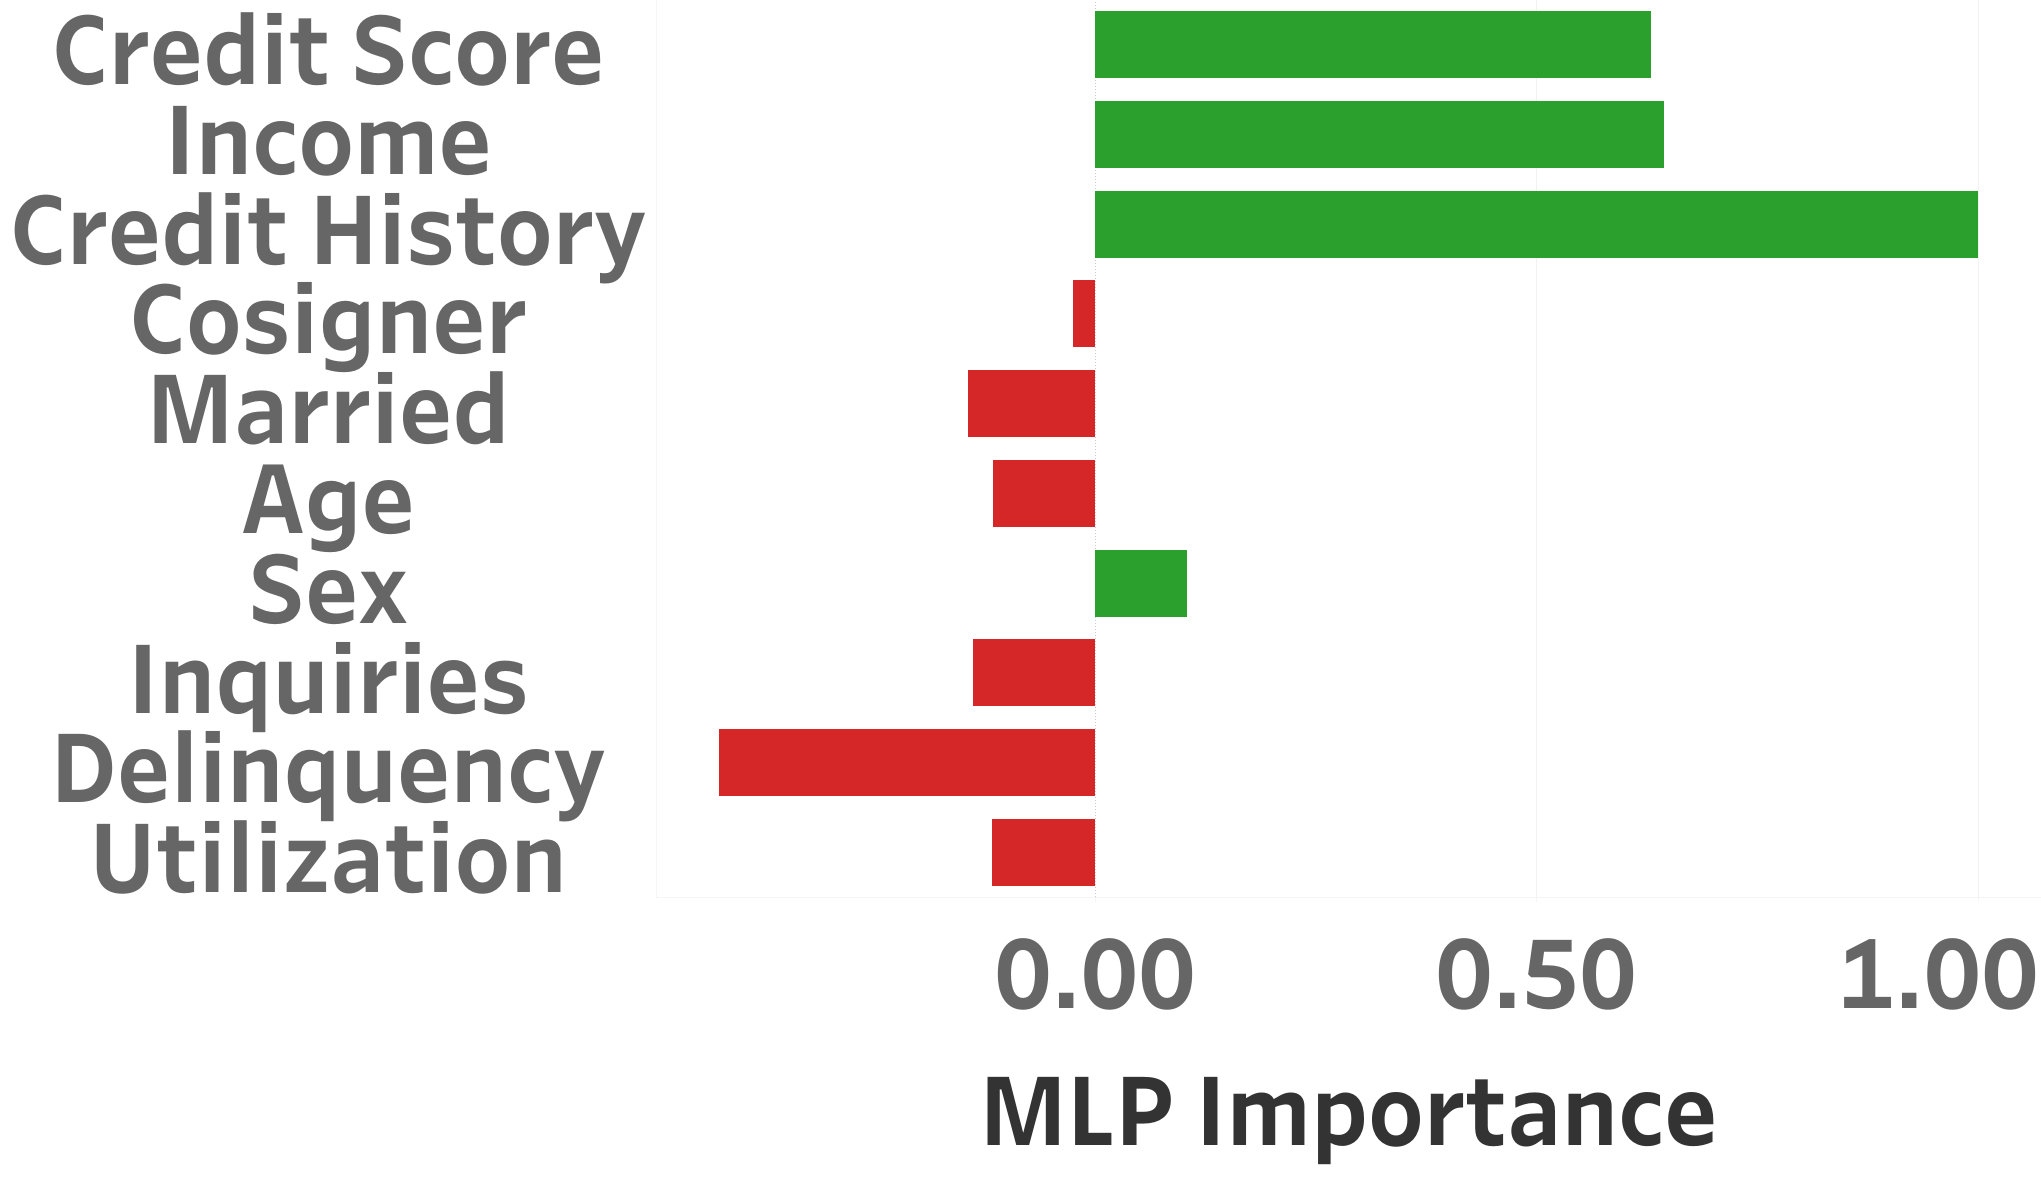
\includegraphics[width=.5\textwidth]{Figures/lime_ex.png}
%      \caption{Output of LIME for the denied applicant. The left side indicates $\mathcal{M}$'s probabilities for each class, and the right side quantifies the extents to which LIME says each feature is important to each class.}
%      \label{fig:lime_ex}
%  \end{figure}


% LIME assigns each a feature a numerical measure of importance to predictions by $\mathcal{M}$. The most important features can be deduced by considering the magnitude of each feature importance value. An ``average explanation" additionally be obtained by averaging these values over the test-set.  Since LIME also builds a linear model locally for each focal instance, the coefficients of LIME and the ground-truth coefficients can be compared to evaluate how faithful LIME is to the ground truth.
% Figure \ref{fig:lime_ex} shows LIME's explanation for the applicant. This explanation representation exemplifies one of the main criticisms of LIME mentioned in \citep{dieber20assessing}; it is unclear what the values associated to each feature in the rightmost part of the figure mean. The prediction probabilities on the left side tell us that $\mathcal{M}$ predicted that the individual would be rejected with probability $.12$ and accepted with probability $0.88$. LIME standardizes the data (through the transformation $\frac{x-\bar{x}}{\sigma}$) and reports the coefficients of a linear surrogate model (a ridge regressor) trained in a simulated neighborhood of the standardized input of interest. Therefore, feature coefficients on the right side of Figure \ref{fig:lime_ex} are just the surrogate model coefficients and can be taken to be scale-agnostic feature important metrics. We denote them by $\beta^{LIME}$. The value of .31 associated with credit score in Figure \ref{fig:lime_ex} indicates that their credit score was the most important feature for this individual's approval and increasing their credit score by one standard deviation would have increased the output of the ridge regressor by .31. Overall, including the intercept term, the formula for the ridge regressor is as follows. We have abused notation by omitting any indication that the features are standardized. 

% \begin{gather*}
%     LIME(x)=.667 -.002\cdot \text{age} -.001\cdot \text{sex} + .004 \cdot \text{married} +.024 \cdot \text{cosigner} +.101 \cdot \text{credit history} \\+.184 \cdot \text{income} - .072 \cdot \text{utilization} -.047 \cdot \text{delinquency} - .030 \cdot \text{inquiries} +.308 \cdot \text{credit score}
% \end{gather*}


% The ground truth feature importance is represented by $\sigma_i$, where $\beta_i$ are the logistic regression coefficients from Equation 1.  $\beta_i$ are scale-agnostic feature importance measures because the logistic regression takes standardized data as input. $\beta_i$ measures how the odds of loan approval increases when feature $i$ is increased by one standard deviation. Since these coefficients are not directly comparable to LIME's feature coefficients $\beta^{LIME}$ (logistic regression coefficients are interpreted in terms of odds while LIME's coefficients are interpreted in terms of the output of a ridge regressor), we instead compare the max-normalized sets of $\beta_i$ and $\beta^{LIME}_i$. The feature importance values are max-normalized in order to emphasize how LIME and $\mathcal{G}$ compare in terms of relative feature importance.

% % \textcolor{red}{For figure 3, show an example for one rejected applicant and one approved applicant; use the same order of features in the y-axis}



% Having constructed a model $\mathcal{M}$ and defined a way to compare feature importance between LIME and $\mathcal{G}$, we can apply LIME to $\mathcal{M}$ to attempt to find what features mattered for the applicant's denial. We use feature importance of $\mathcal{G}$ as the ground truth to compare with the feature importance generated by post hoc explanations since, in practice, users do not have access to $\mathcal{G}$. The left most image in Figure \ref{fig:loan_pipeline} compares LIME's relative feature importance values for the applicant with those of $\mathcal{G}$. 
% Logistic Regression has a value of 1 for credit score, indicating that in reality, credit score is the most important feature and has a positive relationship with the probability of approval. LIME also has a value of 1 for credit score, meaning that it has successfully identified that both that credit score is the most important feature and that it has a positive relationship with loan approval probability. However, LIME provides an incorrect view of the order of importance and impact of the remaining features. Notably, LIME suggests that the number of credit inquiries is the second most important feature despite it actually only being the sixth most important feature. 


% \subsection{Prescriptive Insight}
% \label{sec:prescriptive}
%      Now we demonstrate a simple way to leverage LIME to obtain guidance for denied applicants who would like to be approved in the future. We produce counterfactuals with LIME by simply perturbing the most important feature it identifies. This time, we consider another applicant whose loan application is rejected and check if LIME can provide effective guidance for how to make the applicant's next application be approved. The applicant in question is a 39-year-old married male who has a cosigner, a credit score of 672, and makes \$38,771/year. They have a 20-month-old line of credit, use 20\% of their total credit, have had 5 credit inquiries in the past 6 months, and it has been 21 months since their last delinquent payment. Figure \ref{fig:lime_negative_ex} shows LIME's feature importance values for the denied applicant. LIME implies that the top three most important factors for their rejection were their number of recent credit inquiries, income, and the time since the last delinquent payment. We suppose that the individual would like to just wait some time for their credit inquiries to disappear off of their report, but does not know how many of the five inquiries they have that they need to erase. Manual perturbation of the number of credit inquiries showed that $\mathcal{M}$ would accept their application if their number of credit inquiries is reduced by at minimum two standard deviations. However, even setting the number of credit inquiries to zero does not yield an application that $\mathcal{G}$ would accept. 


% In the next two sections, we will investigate and show evidence why post hoc explainers could lead to wrong descriptive and prescriptive insights. Specifically, we focus on two aspects of post hoc explanations, namely, the \textit{correctness} and \textit{multiplicity}.   The following subsections document various vulnerabilities in these two aspects post hoc explainers have and how they could cause business researchers to misunderstand a business process. 




\section{Incorrectness of Post Hoc Explanations}
    In this section, we investigate the correctness of managerial insights derived from post hoc explanations. Correctness of an explanation refers to the extent an explanation faithfully reflects the underlying phenomena in the data. Obtaining correct insights is the fundamental goal of the \pipeline. % We will explore whether post hoc explainers can provide useful descriptive and prescriptive insights on average. We then identify properties of the data, model, and explainers that lead to incorrect explanations and demonstrate how those effects individually affect explanation quality. 
% REMOVED FOR CIST    
%Finally, we investigate whether some mitigation methods work.


            \subsection{Unfaithful Descriptive Insights}
                    \label{sec:unfaithful_descriptive}
                    
                     % we  check if post hoc explanations can reproduce the correct feature importance rankings from an interpretable model. To do this, we first train a highly accurate logistic regression model on the loan approval data set. We replace the target column with the output of the logistic regression model so that the data can be viewed as being generated by the model. The coefficients of the model then provide a known ground truth feature importance ranking that enable us to 
%To assess how well LIME and SHAP can provide managers with useful descriptive insights, 
We first investigate how faithful LIME and SHAP explanations are to $\mathcal{G}$ to set a baseline expectation for the trustworthiness of post hoc explainers. We obtain the feature importance values from LIME and SHAP  by inspecting the coefficients of their (underlying) models\footnote{We assume that both $\mathcal{G}$ and $\mathcal{M}$ assign social support an importance of 0 and do not allow $\mathcal{M}$ to observe it. Social support is not used directly to determine loan approval probability and is only important insofar as it affects features which \emph{are} used directly.}.  First, we assess how well LIME and SHAP rank the features from most detrimental to loan approval to most beneficial to loan approval. Second, we assess how often LIME and SHAP correctly identify the top $K$ features (regardless of order) for varied $K$. This is because, in practice, it may often be sufficient to find the top $K$ most important features. %For example, with a practical data set consisting of many features, say a hundred, users may just wish to find the top 5 most important features from among them.

%For both the evaluations above, we measure the correctness and consistency of feature importance rankings of LIME and SHAP using the notion of Spearman Rank Correlation \citep{MyersJeromeL2010Rdas}.%Supposing that a data set has $K$ features which has two sets of feature rankings $R_1$ and $R_2$, respectively, the Spearman Rank Correlation between these rankings is $r_s = 1 - \frac{6\sum_k (R_{1,k} - R_{2,k})^2}{K(K^2-1)}$. 
%If $r_s$ is positive and near $1$ it means that the two sets of feature rankings trend together, while if $r_s$ is negative and near $-1$ it means that the two sets of feature rankings trend in opposite directions. If $r_s$ is near 0, it means that the feature rankings are weakly correlated. %We use Spearman Correlation to assess 1) how well LIME and SHAP explanations align with the ground truth, and 2) how consistent LIME and SHAP are with each other. 
                     
 %In Section \ref{sec:relative_importance}, we will compute the Spearman Rank Correlations between the ground truth feature ranking in $\mathcal{G}$ (formula \ref{eqn:gt}) and those given by LIME and SHAP for 100 randomly sampled loan applicants. If the post hoc explanations are 100\% correct, then the correlation should be 1. Any value less than 1 indicates an error in the ranking, leading users to misinterpret the importance of some features. %Then, in the following section, we assess how well LIME and SHAP find the correct signs of importance of the features. Such is important because, e.g., if LIME recognizes the importance of age in relation to the other features, but tells users that age has a negative relationship with loan approval probability, older applicants could incorrectly suspect ageism. 



                    \subsubsection{Identifying Relative Importance and Effect of Features}
                        \label{sec:relative_importance}
 We can tell the relative importance and effects of features from LIME by inspecting the magnitudes and signs (respectively) of its surrogate model's coefficients. This is done similarly for SHAP by inspecting the magnitudes and signs of its Shapley values. Using feature importance values from LIME and SHAP and the coefficient values from $\mathcal{G}$ in Equation \ref{eqn:gt} we can compare the feature importance rankings from LIME, SHAP, and $\mathcal{G}$ using Spearman rank correlations \citep{MyersJeromeL2010Rdas} between the rankings of the explainers' importance values and the ranking of coefficient values from $\mathcal{G}$.  If Spearman rank correlation is 1 means the two input rankings are the same. If it is -1, they are the reverse of each other. If it is 0, the two rankings are uncorrelated. Thus, any correlation less than 1 indicates an error in the ranking, leading users to misunderstand the importance or role of some features. 
 
                        
        We evaluate LIME and SHAP by checking their Spearman rank correlations for rankings of 100 applicants in the test set. Figure \ref{fig:lime_shap_Spearman_signed} shows violin plots of Spearman rank correlations of the ranked feature importance values from LIME/SHAP and $\mathcal{G}$. LIME has a tradeoff between having strong positive median correlation and outliers with a strong negative correlation. SHAP, in contrast, consistently produces rankings that are weak or uncorrelated with the true ranking.
                        
        \paragraph{Discussion}
        These results suggest that when managers attempt to use LIME to find how features affect the outcome of interest, LIME may tell them that the features have the opposite of their true effect. SHAP, on the other hand, may not be useful for finding what features are important because its rankings usually have low correlation with the ground truth ranking. Both LIME and SHAP seem to have difficulty reliably ranking features and identifying how they affect the target variable.


                        

        % REMOVED FOR CIST
        %             \subsubsection{Identifying Signed Importances}
        %                 \label{sec:signed_importance}
        %                 We extend the experiment of the previous subsection by ranking signed feature importance values instead of just magnitudes. This measures the respective abilities of LIME and SHAP to not only identify what the most important features are, but also how they impact the target variable.
        %                 %LIME assigns each a feature a numerical measure of importance to predictions by $\mathcal{M}$. We deduce what features are the most important by considering the magnitude of each feature importance value. We can additionally obtain an ``average explanation" by averaging these values over the test-set. 
        %                 Figure \ref{fig:lime_shap_Spearman_signed} shows violin plots of Spearman rank correlations for the classification of signed feature importance values from LIME and SHAP against those of $\mathcal{G}$. We find that the mean Spearman rank correlations for LIME actually increase\footnote{This does not seem to be the general behavior of LIME. By decreasing the accuracy of $\mathcal{M}$, LIME behaves like SHAP in that the mean and median Spearman rank correlations for signed importance rankings are less than the ones for unsigned importance rankings.}, but outliers with significant negative correlations appear. With the exception of LIME's ranking of the signed feature importance values, the Spearman rank correlations between LIME and SHAP and the ground truth rankings are consistently weak. The mean and median rank correlation for SHAP decreases slightly when going from ranked importance magnitudes to ranked signed importances, and the variance of the ranking distribution increases compared to the results for relative importance. 

        %                 Figure \ref{fig:lime_shap_Spearman_signed_mag}, in short, shows that LIME and SHAP could not rank features related to loan approval in accordance with the true ranking. This shows concretely the potential for users of LIME and SHAP to be misled by their explanations. 

        % \begin{figure}[ht!]
        %     \centering
        %     \begin{subfigure}{.5\textwidth}
        %       \centering
        %       \captionsetup{justification=centering}
        %       \includegraphics[width=.9\linewidth]{Figures/lime_shap_Spearman_magnitude.png}
        %       \caption{Spearman rank correlations of ranked feature importance magnitudes from LIME and SHAP against the true ranked magnitudes from $\mathcal{G}$.}
        %        \label{fig:lime_shap_Spearman_magnitude}
        %     \end{subfigure}%
        %     \begin{subfigure}{.5\textwidth}
        %       \centering
        %        \captionsetup{justification=centering}
        %       \includegraphics[width=.9\linewidth]{Figures/lime_shap_Spearman_signed.png}
        %       \caption{Spearman rank correlations of signed feature importance magnitudes from LIME and SHAP against the true ranking from $\mathcal{G}$.}
        %        \label{fig:lime_shap_Spearman_signed}
        %     \end{subfigure}
            
        %     \caption{Violin plots of Spearman correlations between LIME and SHAP feature importance rankings, both signed and unsigned, against the true rankings. }
        %    \label{fig:lime_shap_Spearman_signed_mag}
        %\end{figure}
                        %                        only compare the top K features 
                    %    out of the topK that LIME or SHAP identifies, how many (compute percentage) are indeed the top K? Report the violinplot for K going from 1 to the total number of features (when K = the total number of features, recall should be 1)
                    % GIVE DEFINITION OF RECALL
                    \subsubsection{Recall of the Most Important Features}
                        The previous section explores the abilities of LIME and SHAP to recover correct importance information about all features used by $\mathcal{G}$, but in practice  users may only care about, say, the top 3 most important features. Finding the top $K$ most important features to a model is one of the most common use cases for LIME and SHAP. This being the case, we now investigate the abilities of LIME and SHAP to correctly identify the top $K$ features (regardless of order or sign). 
                        
                        Our investigation tasks LIME and SHAP with explaining application decisions by $\mathcal{M}$ and computing, for $K=1,2,3\ldots,\text{Number of Features}$,  the average recall of the top $K$ features over 100 applicants in the test set. The same $\mathcal{M}$ as in the previous section is used here. The recall, or true positive rate, represents in this context the true positive rate for the identification of what features are among the top $K$ most important to $\mathcal{G}$ according to $\mathcal{M}$ and $\mathcal{E}$. 
                        
                        The results are shown in Figure \ref{fig:avg_recall}. The results for $K=1,2,3$ show that LIME and SHAP can only correctly identify the top 3 most important features about 40-55\% of the time. %LIME has a recall of 1 for $K=5,6$ but not $K=1,2,3,4$ because it cannot always order the top $4$ features correctly. Both LIME and SHAP can correctly identify the top 4 features about 80\% of the time. 

                        \paragraph{Discussion}
                        The fact that LIME and SHAP cannot identify the top  features reliably should urge business researchers to use them with caution for this purpose. Suppose, for example, a firm trying to increase customer retention sees that LIME identifies ad spending as the most important feature when it actually is not. The firm could waste resources needlessly buying ads.

    % removed for cist
    % \subsubsection{Discussion} 
    %     The results of this section are meant to give insights into how LIME and SHAP serve users in finding descriptive insights a practical business application. Figure \ref{fig:lime_shap_Spearman_signed_mag} showed a scenario where the two most popular post hoc explainers (LIME and SHAP) could not correctly order features in terms of how important they are and how they affect the outcome variable. In our scenario, we had a realistic data set with 5000 data points and explained a black-box model trained on that data set that had a test set accuracy of 85\%. 
% REMOVED FOR CIST        
%We will show in Section \ref{sec:m_fidelity} that we can reach similar conclusions when the data size and accuracy of $\mathcal{M}$ are varied.

    \subsection{Unfaithful Prescriptive Insight}
        \label{sec:actionable_recourse}
        Since Section \ref{sec:unfaithful_descriptive} showed that LIME and SHAP may fail both to correctly indicate what features are most important to loan approval and how the features affect loan approval probability, this section will show that they may additionally fail to be useful in advising how to change features to obtain more desirable outcomes. We substantiate the claim that changing the most important feature(s) to an outcome identified by LIME or SHAP is unlikely to change the outcome. 
        
        We test two ways to obtain post hoc prescriptive insights. %We now investigate whether the most important features identified by LIME and SHAP are actionable. Both LIME and SHAP can indicate that certain features are relatively important to $\mathcal{M}$'s output compared to the others, but do not advise how to change those features in order to change $\mathcal{M}$'s output. The following example highlights a deficiency with such explanations. Supposing that LIME indicated that a rejected applicant's credit history key to their rejection, the applicant would naturally wonder if waiting a year would allow them to be approved. If not, this puts into question the sense in which the length of the credit history was important. Users need a system to propose actions they can take to improve their outcome. In this paper, we will consider two ways to construct such a system. 
        The first way is the naive way \textemdash we manually perturb important features identified by LIME and SHAP until a counterfactual is found. The second way is to use a dedicated counterfactual explainer such as DiCE.

            
        In our simulation experiment, we suppose that applicants use an MLP $\mathcal{M}$ trained on our data set to be able to anticipate banks' loan approval decisions. We consider the situation where rejected individuals would like to find out how to be approved in their next application. They do this using LIME and SHAP to explain the aforementioned MLP decision using their data as inputs. We wish to find how often LIME, SHAP, and DiCE can produce new application profiles for rejected applicants that both $\mathcal{M}$ and $\mathcal{G}$ will accept. We refer to such counterfactual examples as \emph{true counterfactuals}. 

            
        To test LIME and SHAP's ability to produce true counterfactuals, we perturb the top $K$ most important features of 100 denied applicants in the loan approval test set (as seen by LIME and SHAP) and track the percentage of true counterfactuals that LIME and SHAP can produce.  Application profiles are changed by perturbing the top $K=1,2,3,4$ features by multiples of 10\% of their standard deviations, up to a full standard deviation. Since DiCE perturbs inputs automatically, we vary the number of features it is allowed to perturb to create counterfactuals and again track the percentages of true counterfactuals it creates.
            
            
            %Our  experiment is repeated four times by setting $K=1,2,3,4$. We use the same data as in the previous section. This is similar to the experiment used in \citep{kommiya21towards} to show that the top features identified by LIME and SHAP to predict hospital admissions are not sufficient to produce counterfactuals. The results are recorded in Figures 3-5.  





        
 %\tw{Ronilo experiment: allow changing top K features and report the successful recourse for LIME and SHAP}           
            Figures \ref{fig:lime_recourse_k} and \ref{fig:shap_recourse_k} plot the perturbation extent versus the proportion of times 100 previously rejected applicants got approved by both $\mathcal{M}$ and $\mathcal{G}$ for LIME and SHAP, respectively. Following intuition, increasing the number of features that can be perturbed and increasing the extents to which those features can be perturbed increases the likelihood of being able to produce true counterfactuals for both LIME and SHAP. However, although larger perturbations generally lead to increasing proportions of approvals, in general only a minority of individuals ($\leq$ 50\%) will be approved using recourse recommended by either LIME or SHAP. 
            
            Results for DiCE appear in Figure \ref{fig:dice_recourse_k}. Since DiCE automatically selects what features to tune and how much to vary them for counterfactual generation, we prevent it from changing individuals' sex and marital status. Interestingly, DiCE's performance is significantly worse than those of LIME and SHAP, with a maximum of about a 12\% success rate. 

            \paragraph{Discussion}
            Although post hoc explainers may seem to present a way to develop interventions or provide explanations to customers or stakeholders via counterfactual generation, doing so does not seem to be straightforward. \citep{kommiya21towards} even shows, counter-intuitively, that using all but the top features identified by LIME and SHAP is the most reliable way to generate counterfactuals. Thus, it is difficult to recommend using either of them for counterfactual generation. Likewise, we are hesitant to recommend DiCE due to its low success rate.

        % % allow tuning of DiCE sparsity_weight
        % \subsubsection{Recourse via Counterfactual Explainer}
        %     \label{cf_recourse}
        %     A dedicated counterfactual explainer such as DiCE should be used over LIME and SHAP for counterfactual generation. We will show that even when LIME and SHAP are successful in creating counterfactuals $x'$ from a point $x$, their counterfactuals are often more different than $x$ than the ones from DiCE to motivate this claim. To motivate the utility of close counterfactuals using our loan approval example, consider that denied applicants will of course want to make \emph{minimal} changes to their behavior in their quests to be approved in their next applications. 
%\tw{Feng Lu experiment \# 4: generate DiCE counterfactuals for 1000 data points for model M, and report the percentage of success that the counterfactuals get a different label from G}

 


        % \paragraph{Comparison of Counterfactual Distances between LIME, SHAP, and DiCE}
        
        % To compare the closeness of the counterfactuals produced by LIME, SHAP, and DiCE. We find a set of 100 points $x$ for which LIME, SHAP, and DiCE can successfully create counterfactuals $x'$.  For each explainer, we plot a violin plot for the resulting distances $\norm{x-x'}_2$. The results of this experiment appear in Figure \ref{fig:cf_perturb}. Figure \ref{fig:cf_perturb} shows that the median and mean counterfactual distances are lower for DiCE than it is for either LIME or SHAP, implying that DiCE, on average, asks less of individuals when providing means of recourse. By comparing the inner box plots of the violin plots in Figure \ref{fig:cf_perturb}, we can also see that the box plot for DiCE has a lower IQR than those of LIME and SHAP. Hence, DiCE also has comparatively less variability.
                    
            
  

            
            % \begin{figure}[ht!]
            %     \centering
            %     \includegraphics[width=.5\textwidth]{Figures/lime_shap_dice_dists.png}
            %     \caption{Violin plots of the extents to which LIME, SHAP, and DiCE must perturb data points to produce true counterfactuals.}
            %     \label{fig:cf_perturb}
            % \end{figure}

        % \begin{figure}[ht!]
        %     \centering
        %     \begin{subfigure}{.5\textwidth}
        %       \centering
        %       \captionsetup{justification=centering}
        %       \includegraphics[width=.9\linewidth]{Final_Figures/fig8a.png}%{Figures/feng_fig/sparsity_dice.png}
        %       \caption{Percentages of times DiCE was able to produce true counterfactuals for rejected applicants for different sparsity parameters.}
        %        \label{fig:dice_sparsity}
        %     \end{subfigure}%
        %     \begin{subfigure}{.5\textwidth}
        %       \centering
        %        \captionsetup{justification=centering}
        %       \includegraphics[width=.9\linewidth]{Figures/lime_shap_dice_dists.png}
        %       \caption{Violin plots of the extents to which LIME, SHAP, and DiCE must perturb data points to produce true counterfactuals.}
        %        \label{fig:cf_perturb}
        %     \end{subfigure}
            
        %     \caption{Comparison of successful recourse performance by LIME, SHAP, and DiCE for rejected applicants}
        %     \label{fig:cf_figs}
        %\end{figure}
        % \begin{figure}
        %     \centering
        %     \includegraphics[width=.5\textwidth]{Figures/lime_shap_dice_dists.png}
        %     \caption{Violin plots of the extents to which LIME, SHAP, and DiCE must perturb data points to produce true counterfactuals.}
        %     \label{fig:enter-label}
        % \end{figure}


\section{Multiplicity of Post Hoc Explanations}
        A multiplicity of post hoc explainers refers to situations in which one or more post hoc explainers provide a set of explanations that contains some internal disagreement. Both attributive and counterfactual explainers can yield a multiplicity of explanations.%This may or may not be a problem depending on the use-case. For example, one may want to choose from among a set of explanations based on which explanations most align with domain knowledge. Indeed, the ability to produce diverse counterfactuals for the same input is one of the main features of DiCE. However, 
        We are concerned with cases when the multiplicity of explanations is problematic\footnote{Multiplicity can be desirable. DiCE, for example, seeks to create diverse counterfactuals so that users can pick whichever best suits them.}. Examples of such cases could be when one does not have domain knowledge and does not know what explanation to pick, and/or when there are explanations that contradict each other. In any case, picking a single explanation may be difficult because there is no way to know what explanation is the best. 
        
        Due to problematic explainer multiplicity, researchers cannot just choose one explainer or one explanation. \cite{han22which} introduced a no-free-lunch theorem for post hoc explainers, stating that no one explainer can always provide the best explanation. %This is because for every explainer, there must exist a neighborhood around a data point to be explained such that \emph{another} explainer is a better approximator of the ground truth in that neighborhood.
        \cite{kommiya21towards} also showed that different explainers are either (implicitly) solving entirely different optimization problems or solving the same (or a similar one) differently. %They defined two objectives $\alpha$ and $\beta$ for which different post hoc explainers choose to optimize and do so differently. $\alpha$ captures the ability for an explainer to utilize features that are \emph{necessary} for the outcome being explained. $\beta$ captures the ability for an explainer to utilize features that are \emph{sufficient} to cause the outcome being explained. \cite{kommiya21towards} shows that LIME and SHAP take different approaches for optimizing $\beta$, while counterfactual methods optimize for $\alpha$. 
        Thus, theory suggests that we should not expect LIME, SHAP, or DiCE to be consistent with each other. There will always be problematic multiplicity when using post hoc explainers. With this in mind, we use Sections \ref{sec:conflict_between} and \ref{sec:conflict_within} to demonstrate how business researchers could be misled or confused by post hoc explainers due to multiplicity of explanations. Section \ref{sec:mitigation} proposes and tests some mitigation strategies that try to leverage the multiplicity of explanations. 

       \subsection{Inconsistencies Between Explainers}
        \label{sec:conflict_between}
            %To motivate the use of multiple post hoc explainers, we show that they may explain the same outcome in different ways with differing degrees of accuracy. 
            Conflicting explanations between explainers can lead to a conundrum for researchers. On one hand, users may have to choose from among conflicting explanations and suffer the consequences if they pick a bad explanation. On the other, because each explanation has a modicum of truth, managerial insights drawn from a single explainer may be incomplete or incorrect. %Notably, this is increasingly likely as the data dimension increases \citep{kommiya21towards}. To justify these claims, we demonstrate the inconsistency of LIME and SHAP on the simulated loan data set.%, then show how the inconsistency grows when larger and larger feature subsets are used on the Iranian Housing data set. 
    
            To substantiate these claims, we demonstrate the inconsistency of LIME and SHAP on the simulated loan data set. Given a trained MLP $\mathcal{M}$ on the loan data, we would like to investigate how different LIME and SHAP explanations of the same points are. To this end, we sample 100 test set applicants and obtain feature rankings according to the importance allocated to them by both LIME and SHAP. Figure \ref{fig:lime_shap_spearman_together} shows that, on average, LIME and SHAP most often have rankings are nearly uncorrelated and never strongly correlated. The two modes of Spearman rank correlations between LIME and SHAP rankings appear at .25 and -.25, meaning that LIME and SHAP rankings are usually dissimilar. 
            
            % REWORK NEXT TO PARAGRAPHS
            \paragraph{Discussion}
            These results suggest once more that post hoc explainers should be used with caution. It is up to the user to attempt to either somehow leverage multiple explainers or identify which explainer's results are the most sensible using their domain knowledge. However, in cases where users do not have sufficient domain knowledge, the inconsistency between explainers may be confusing and disruptive.% (and taking care to avoid the biases outlined in Section \ref{sec:human_explainer_interaction}. 

            %Being that it is impossible in practice to know what explainer is the most correct, this experiment illustrates the importance of leveraging multiple explainers to maximize the likelihood that correct insights are drawn. Although \citep{kommiya21towards} recommended this, to the best of our knowledge, exactly how to leverage multiple explainers is an open problem. We treat this problem in Section \ref{sec:mitigation}.
        



    \subsection{Inconsistency from the Same Explainer}
            \label{sec:conflict_within}
             Both LIME and SHAP are designed such that there may be variability in explanations of the same outcome between runs. This section focuses on LIME because it has many hyperparameters. 
             Hyperparameters and sampling are causes of inconsistency between multiple runs of LIME. LIME depends on a random seed, the number of samples to generate around the point to explain, the kernel function (default Gaussian), the kernel width defining the size of the neighborhood around the point to explain, as well as  the hyperparameters of its surrogate model (e.g. LASSO vs RIDGE). Recent papers have confirmed that LIME's hyperparameters can significantly change the explanation of the same outcome \citep{rahnama19shift,visani21stability}.

            % i used signed feature importance vals here
             To demonstrate the inconsistency of LIME  in our simulated loan application context, we create 10,000 different instances of LIME and investigate how consistently they rank the importance of features for a single denied applicant in the test set. The 10,000 instances of LIME are constructed by initializing LIME with pairs of 100 kernel widths and 100 random seeds. The results of this experiment appear in Figure \ref{fig:lime_rankings} and indicate that LIME concentrates the rankings for each feature at one value but admits the possibility of giving each feature much higher or much lower ranks.

             \paragraph{Discussion}
             Two key takeaways from Figure \ref{fig:lime_rankings} are that most features have several small modes in addition to a dominant mode, and all features have a ranking distribution that spans from most inimical to most beneficial. This should alert business researchers to the fact that, depending on hyperparameters, LIME could suggest that highly beneficial features are highly inimical and vice versa. Likewise, it may fail to identify influential features.

            
            % To get an idea of how LIME and SHAP explanations are affected by hyperparameters in a business context, we examine the importance of an applicant's credit score given by different combinations of models and explainers. We evaluate consistency by checking 1) if LIME and SHAP can at least give credit score feature importance values with consistent signs and 2) if those values stay relatively consistent regardless of random seeds or hyperparameters. Simultaneously, we investigate how the accuracy of $\mathcal{M}$ affects explanations. %Section \ref{sec:rashomon_overfitting} will give an overview of how instability affects LIME and SHAP.%and results in inconsistent explanations. 

            % We found that feature importance signs were relatively consistent when explaining only one individual. In particular, if we reuse the same experimental setup as in Section \ref{sec:pipeline_demo} and construct importance value histograms by using LIME and SHAP to explain the predictions of the same applicant 100 times by different models $\mathcal{M}$ and different instantiations of LIME and SHAP with different hyperparameter settings and record the importance of the applicant's credit score (the data set's known most important feature), credit score almost always gets a consistently signed feature importance value by both explainers.  Figure \ref{fig:lime_imp_rejected} shows that for each model, regardless of accuracy, LIME almost always gives credit score a negative feature importance sign. But it also admits the possibility of giving credit score a small positive feature importance sign even for more accurate models. Figure \ref{fig:shap_imp_rejected} shows that SHAP is robust to its random seed being changed, but gives credit score larger Shapley values as the accuracy of $\mathcal{M}$ increases.


        

    \section{Attempted ``Mitigation" Strategies}
    Given the identified issues above, we test whether some intuitive mitigation strategies can improve the quality and consistency of post hoc explanations.  
        \subsection{Attempted ``Mitigation'' Strategies for Incorrectness}
        \label{sec:mitigation} %\textcolor{red}{move this to the end of section 4. this is the mitigation strategy for incorrectness}
            We propose a mitigation strategy based on tuning $\mathcal{M}$. We investigate the relationship between the accuracy of $\mathcal{M}$ and the accuracy of LIME and SHAP's feature importance rankings to isolate the effects of $\mathcal{M}$ on LIME and SHAP.  Our hypothesis is that explanations will be more correct for more accurate models, and so researchers may want to spend extra effort obtaining good models. %We used the local fidelity of LIME's linear surrogate models similarly to investigate its trade-off with stability. 
            %We check whether different averaging strategies might reduce the severity with which LIME and SHAP's feature importance rankings differ from those of $\mathcal{G^*}$. 


            \paragraph{Does High-Accuracy of $\mathcal{M}$ Imply High-Quality Explanations?}
            \label{sec:m_fidelity}
                 We test if controlling for the accuracy of $\mathcal{M}$ can mitigate some error in $\mathcal{E}$ by tuning $\mathcal{M}$ and checking the correctness of explanations from LIME and SHAP. We control the accuracy of $\mathcal{M}$ by creating increasingly accurate instantiations of an MLP. This is done by using a consistent initialization of the MLP weights and training it for increasing numbers of iterations.
                
                The results of our test appear in Figure \ref{fig:acc_increase_metric1_strategy1} and show that the explainers follow intuition by giving increasingly accurate feature rankings as $\mathcal{M}$ becomes for more faithful to $\mathcal{G}$. However, even when $\mathcal{M}$ is 100\% accurate\footnote{Note that $\mathcal{M}$ having 100\% test set accuracy does not necessarily mean that $\mathcal{M}=\mathcal{G}$ in the hypothesis space.}, neither LIME nor SHAP can perfectly rank the features. Thus, no matter the quality of $\mathcal{M}$,  post hoc explanations of $\mathcal{M}$ should not be expected to be correct.
            
                %To answer this question, we use two strategies to control the accuracy of the model. One strategy is to assume that there is enough training data and control the accuracy of the model by varying its parameters. The other strategy is to change the accuracy of the model by varying the size of the training data set with the same model parameters. In our experience, differences in model accuracy due to both of these scenarios are common in the real world. \par
                % Figures 15 to 17 show the performance of the metrics in Sections 4.1.1 to 4.1.3 under the two strategies, respectively. From Figure 15, we can find that the correlation of importance magnitude ranking increases accordingly as the accuracy of the model increases, regardless of the strategy adopted. And the effect of the first strategy is significantly better than that of the second strategy. However, unfortunately, realistically researchers may not have enough training data. Therefore, even though our experimental results show that the post hoc explainer can give a very good explanation in terms of importance magnitude ranking when a very good model is trained with enough data, this is almost non-existent in real life. %From Figure 16 we see that no matter what strategy is adopted to improve the accuracy of the model, there is no large improvement in the signed ranking relevance as the accuracy of the model improves. %In terms of recall, it can be seen from Figure 17 that although LIME and SHAP's recall improves with accuracy under both strategies, the improvement is very limited, with the improvement in recall averaging no more than 20\% when the accuracy is improved from about 55\% to 95\%.\par
                %In summary, although the descriptive insights of post hoc explainers improve somewhat with model accuracy, and even in some extreme cases (sufficient data, good models, appropriate metrics) they can give very good descriptive insights, these improvements are more limited or difficult to generalize in the real world.\par
                %Similarly, we considered the effect of model accuracy on prescriptive insights. We used the metrics in Section 4.2.2 to portray the effect of Dice on prescriptive insights. As can be seen in Figure 18, when the model accuracy improves from 55\% to 95\%, the success rate of counterfactual generation improves from 25\% to 50\%. Despite the degree of improvement in success rate, even the better models do not end up with very good prescriptive insights.


            
                % \begin{figure}[ht!]
                % \centering
                %     \begin{subfigure}{.48\textwidth}
                %           \centering
                %           \includegraphics[width=\linewidth]{Final_Figures/fig14a.png}%{Figures/feng_fig/acc_increase_iter_1.png}
                %           %\caption{A subfigure}
                %           \label{fig:acc_increase_metric1_strategy1}
                %     \end{subfigure}%
                %     \hfill
                %     \begin{subfigure}{.48\textwidth}
                %           \centering
                %           \includegraphics[width=\linewidth]{Final_Figures/fig14b.png}%{Figures/feng_fig/acc_increase_size_1.png}
                %           %\caption{A subfigure}
                %           \label{fig:acc_increase_metric1_strategy2}
                %     \end{subfigure}
                %     \hfill
                % \caption{Line plots of 100 Spearman rank correlations of feature importance magnitude ranking given by LIME and SHAP when increasing $\mathcal{M}'s$ accuracy by changing model parameter strategy (left) and changing training size (right) strategy. Vertical lines indicate the 95\% confidence interval of the Spearman correlation for given accuracies.}
                % \label{fig:acc_increase_metric1}
                % \end{figure}
        \subsection{Attempted ``Mitigation'' Strategy for Inconsistency} 
        \label{sec:inconsistency_mitigation}
            Section \ref{sec:conflict_within} demonstrated the multiplicity of explanations due to random seeds and hyperparameters, so it is natural to wonder if the multiplicity of explanations can be leveraged via an averaging strategy.
            
            \subsubsection{Does Averaging Explanations of One Explainer Yield Better Explanations?}
                We check if taking the mean of feature importance values from multiple instances of LIME and SHAP taken over combinations of random seeds and hyperparameters reveals a useful aggregation strategy. Figure \ref{fig:avering_within_lime_metric1} shows that when averaging over increasing numbers of instances of LIME, the quality of the resulting explanations does not improve, but the variability does decrease somewhat (note the internal box plots). Figure \ref{fig:avering_within_shap_metric1} shows that such averaging with SHAP has no effect. It is not clear that aggregating the results of one type of explainer is useful. 
                % \begin{figure}[ht!]
                % \centering
                %     \begin{subfigure}{.48\textwidth}
                %           \centering
                %           \includegraphics[width=\linewidth]{Final_Figures/fig22a.png}%{Figures/feng_fig/lime_0_v1.png}
                %           %\caption{A subfigure}
                %           \label{fig:avering_within_lime_metric1}
                %     \end{subfigure}%
                %     \hfill
                %     \begin{subfigure}{.48\textwidth}
                %           \centering
                %           \includegraphics[width=\linewidth]{Final_Figures/fig22b.png}%{Figures/feng_fig/shap_0_v1.png}
                %           %\caption{A subfigure}
                %           \label{fig:avering_within_shap_metric1}
                %     \end{subfigure}
                % \caption{Violin plots of 100 Spearman rank correlations of feature importance magnitude ranking given by LIME (left) and SHAP (right) when averaging different numbers of model results}
                % \label{fig:avering_within_experlainers_metric1}
                % \end{figure}
  
    
            

            
            % \begin{figure}[ht!]
            %     \centering
            %     \includegraphics[width=.5\textwidth]{Final_Figures/fig21.png}%{Figures/feng_fig/average_lime_shap_3_v1.png}
            %     \caption{Average recall of LIME, SHAP and LIME+SHAP}
            %     \label{fig:lime_shap_Spearman_together}
            % \end{figure}
            
            
            % \begin{figure}[ht!]
            % \centering
            %     \begin{subfigure}{.48\textwidth}
            %           \centering
            %           \includegraphics[width=\linewidth]{Final_Figures/fig22a.png}%{Figures/feng_fig/lime_0_v1.png}
            %           %\caption{A subfigure}
            %           \label{fig:avering_within_lime_metric1}
            %     \end{subfigure}%
            %     \hfill
            %     \begin{subfigure}{.48\textwidth}
            %           \centering
            %           \includegraphics[width=\linewidth]{Final_Figures/fig22b.png}%{Figures/feng_fig/shap_0_v1.png}
            %           %\caption{A subfigure}
            %           \label{fig:avering_within_shap_metric1}
            %     \end{subfigure}
            % \caption{Violin plots of 100 Spearman rank correlations of feature importance magnitude ranking given by LIME (left) and SHAP (right) when averaging different numbers of model results}
            % \label{fig:avering_within_experlainers_metric1}
            % \end{figure}
            
            
            % \begin{figure}[ht!]
            % \centering
            %     \begin{subfigure}{.48\textwidth}
            %           \centering
            %           \includegraphics[width=\linewidth]{Final_Figures/fig23a.png}%{Figures/feng_fig/lime_1_v1.png}
            %           %\caption{A subfigure}
            %           \label{fig:avering_within_lime_metric2}
            %     \end{subfigure}%
            %     \hfill
            %     \begin{subfigure}{.48\textwidth}
            %           \centering
            %           \includegraphics[width=\linewidth]{Final_Figures/fig23b.png}%{Figures/feng_fig/shap_1_v1.png}
            %           %\caption{A subfigure}
            %           \label{fig:avering_within_shap_metric2}
            %     \end{subfigure}
            % \caption{violin plots of 100 Spearman rank correlations of signed feature importance rankings given by LIME(left) and SHAP(right) when averaging different numbers of model results}
            % \label{fig:avering_within_experlainers_metric2}
            % \end{figure}
            
            % \begin{figure}[ht!]
            % \centering
            %     \begin{subfigure}{.48\textwidth}
            %           \centering
            %           \includegraphics[width=\linewidth]{Figures/feng_fig/lime_2_v1.png}
            %           %\caption{A subfigure}
            %           \label{fig:avering_within_lime_metric3}
            %     \end{subfigure}%
            %     \hfill
            %     \begin{subfigure}{.48\textwidth}
            %           \centering
            %           \includegraphics[width=\linewidth]{Figures/feng_fig/shap_2_v1.png}
            %           %\caption{A subfigure}
            %           \label{fig:avering_within_shap_metric3}
            %     \end{subfigure}
            % \caption{Average recall given by LIME(left) and SHAP(right) when averaging different numbers of model results}
            % \label{fig:avering_within_experlainers_metric3}
            % \end{figure}
            
            \subsubsection{Does Averaging Explanations Across Explainers Yield Better Explanations?}
                Noting the inconsistency between explainers, we test the efficacy of averaging feature importance rankings from LIME and SHAP together. We produce explanations for 100 applicants using default LIME and SHAP instances, then average the LIME and SHAP explanations for each applicant. We compare the quality of these explanations in Figure \ref{fig:averaging_lime_shap}.  

                It is also unclear from Figure \ref{fig:averaging_lime_shap} whether aggregating LIME and SHAP is beneficial. The most accurate explanation from LIME and SHAP combined is better than the best from LIME but worse than the best from SHAP. The variance of the quality of explanations LIME and SHAP combined is comparatively larger than LIME's and comparatively lower than SHAP's. 


% \begin{figure}[!htb]
% \minipage{0.32\textwidth}
%   \includegraphics[width=\linewidth]{Final_Figures/fig22a.png}
%   %\label{fig:avering_within_lime_metric1}
%   \caption{Violin plots of 100 Spearman rank correlations of LIME feature importance magnitude rankings when averaging different numbers of model results}\label{fig:avering_within_lime_metric1}
% \endminipage\hfill
% \minipage{0.32\textwidth}
%   \includegraphics[width=\linewidth]{Final_Figures/fig22b.png}
%   %\label{fig:lime_recourse_k}
%   \caption{Violin plots of 100 Spearman rank correlations of LIME feature importance magnitude rankings when averaging different numbers of model results}
%   \label{fig:avering_within_shap_metric1}
% \endminipage\hfill
% \minipage{0.32\textwidth}%
%   \includegraphics[width=\linewidth]{Final_Figures/fig20.png}
%   %\label{fig:dice_recourse}
%   \caption{Violin plots of Spearman Rank Correlations of feature importance magnitude ranking by LIME, SHAP and LIME+SHAP}
%   \label{fig:lime_shap_Spearman_together}
% \endminipage
% \end{figure}



                
                
                % \begin{figure}[ht!]
                %     \centering
                %     \includegraphics[width=.5\textwidth]{Final_Figures/fig20.png}%{Figures/feng_fig/average_lime_shap_1_v1.png}
                %     \caption{Violin plot of Spearman Rank Correlations of feature importance magnitude ranking by LIME, SHAP and LIME+SHAP}
                %     \label{fig:lime_shap_Spearman_together}
                % \end{figure}
            % \begin{figure}[ht!]
            % \centering
            %     \begin{subfigure}{.48\textwidth}
            %       \centering
            %       \includegraphics[width=\linewidth]{Final_Figures/fig15a.png}%{Figures/feng_fig/acc_increase_iter_2.png}
            %       %\caption{A subfigure}
            %       \label{fig:acc_increase_metric2_strategy1}
            %     \end{subfigure}%
            %     \hfill
            %     \begin{subfigure}{.48\textwidth}
            %       \centering
            %       \includegraphics[width=\linewidth]{Final_Figures/fig15b.png}%{Figures/feng_fig/acc_increase_size_2.png}
            %       %\caption{A subfigure}
            %       \label{fig:acc_increase_metric2_strategy2}
            %     \end{subfigure}
            % \caption{Line plots of 100 Spearman rank correlations of signed feature importance magnitude given by LIME and SHAP when increasing $\mathcal{M}'s$ accuracy by changing model parameter strategy (left) and changing training size (right) strategy.}
            % \label{fig:acc_increase_metric2}
            % \end{figure}
    
    
    
    
    
            
% REMOVED FOR CIST
% \subsection{Why post hoc Explanations Are Incorrect}
% Having shown that, on average, LIME and SHAP cannot reliably produce accurate descriptive or prescriptive insights for managers, we proceed with a systematic analysis of the causes of failures of post hoc explainers. The analysis proceeds in two parts, corresponding to the two stages identified in Figure \ref{fig:pipeline}. In our analysis, we posit the existence of an unknown data generator $\mathcal{G}$ and a sufficiently good black-box approximator of $\mathcal{G}$ labeled $\mathcal{M}$. We will assume, for the sake of our analysis, that no glass-violin approximator is available. We then identify and presuppose the conditions necessary for a post hoc explainer to be effective, and examine the consequences of those conditions being met and not met. Finally, we propose and test several mitigation strategies that those involved with post hoc explainers can use.


% \subsubsection{Stage 1 Issues: The Effects of Multicollinearity, Confounding, Unobserved Features}
%     \label{sec:data_related_issues}
%     We assume that managers, using post hoc explainers, want to deduce causal relations about $\mathcal{G}$ from $\mathcal{M}$. The two general preconditions for this are that the data collected from $\mathcal{G}$ satisfy a set of conditions necessary for causal inference and that $\mathcal{M}$ is properly specified. In practice, though, it is unreasonable to ever expect that a data set would have no multicollinearity, no confounding features, and no unobserved features. Indeed, our data set fails these conditions because social support is an unobserved confounder of the cosigner feature. 
    
%     In our first set of experiments, we examine the individual effects of multicollinearity, confounding, and unobserved features on LIME and SHAP explanations. To isolate the individual effects, we will create an ideal data generator $\mathcal{G}^*$ together with a problematic data generator for each effect. $\mathcal{G}^*$ generates data that satisfies causal inference conditions. The problematic data generator will be labeled $\mathcal{G}_{\text{effect}}$, where "effect" is the effect of interest, and will have that effect as its sole violation of causal inference conditions. We then compare the abilities of LIME and SHAP to explain $\mathcal{G}^*$ and $\mathcal{G}_{\text{effect}}$ for each effect. We also consider an ideal situation where we use a data generator that satisfies causal inference $\mathcal{G}^*$, and compare the abilities of LIME and SHAP to explain both $\mathcal{G}^*$ directly and a highly accurate MLP model $\mathcal{M}$ trained on the data from $\mathcal{G}^*$. 

%     In this section, the model data generator $\mathcal{G}^*$ uses a simplified set of features. Namely, age, sex, credit inquiries, credit utilization, credit score, and availability of a cosigner. All features are independent of each other. When training the models $\mathcal{M}$ on $\mathcal{G}^*$ and $\mathcal{G}_{\text{effect}}$, we again have the setup where 5000 applicants are generated and $\mathcal{M}$ is a perceptron. For each experiment, $\mathcal{M}$ has 3-5 hidden layers and is trained for sufficiently many iterations so that its ROC AUC is between 80\% and 85\%. 
    
%     %With enough observations, you will eventually be able to identify the separate effects of even highly collinear (but never perfectly collinear) variables. This is why Rob Franzese and UMich likes to call multicollinearity "micronumerosity."


%     \paragraph{Collinear Features}
%     If two features are highly correlated, it can be difficult to ascertain the extents with which the two features have causal effects on an outcome. Multicollinearity is especially problematic in data with small sample sizes. We illustrate the effect of collinearity on explanations as follows. Suppose that we construct $\mathcal{G}_{colinear}$ by altering $\mathcal{G}^*$ such that credit score becomes a linear function of age:
%     %http://www.themoneyalert.com/credit-score-rating-scale-range/
%         \begin{equation*}
%             \text{credit score} = 2.2 \cdot \text{Age} + (105-100)\cdot \text{Utilization} + \epsilon
%         \end{equation*}

%     where $\epsilon \sim \mathcal{N}(500, 70)$. This model reflects that, on average, credit scores increase with age and decrease with utilization. We hypothesize that because age, utilization, and credit score are collinear, LIME and SHAP will have some difficulty disambiguating their feature importances. 

%     We then explain 100 application decisions from $\mathcal{G}^*$ and $\mathcal{G}_{\text{colinear}}$ with LIME and SHAP, and compare violin plots of the Spearman rank correlations of the ranked feature importance magnitudes provided by LIME and SHAP and the ground truths. Figure \ref{fig:lime_colinear} shows that, without collinearity, LIME can almost always correctly order the features by importance. When collinearity is added by making credit score depend on age and utilization, LIME can no longer do this; the variance of the rankings increases. SHAP's results, shown in Figure \ref{fig:shap_colinear}, show that adding collinearity to the data greatly increased the variance of the rankings and significantly lowered both the mean and median rank correlation. The IQR of the Spearman rank correlations for SHAP seems to nearly double in the presence of collinearity in this case. SHAP evidently loses the ability to perfectly rank the features because the upper tail of the Spearman rank correlation distribution goes down to about .75. 

%         \begin{figure}[ht!]
%             \centering
%             \begin{subfigure}{.5\textwidth}
%               \centering
%               \captionsetup{justification=centering}
%               %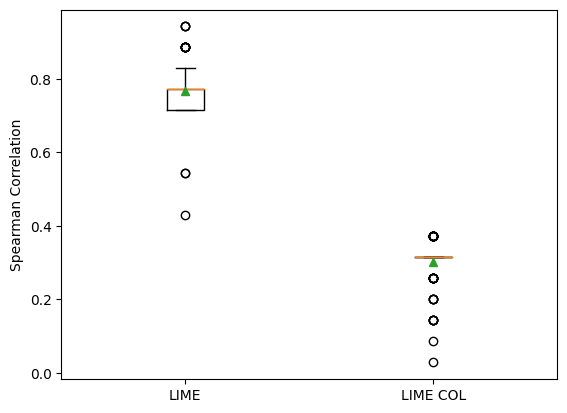
\includegraphics[width=.9\linewidth]{Figures/lime_colinearity.png}
%               \includegraphics[width=.9\linewidth]{Final_Figures/fig9a.png}%{Figures/lime_spearman_colinear.png}
%               \caption{}%Spearman rank correlations of ranked feature importance magnitudes from LIME against the true ranked magnitudes from $\mathcal{G}$.}
%                \label{fig:lime_colinear}
%             \end{subfigure}%
%             \begin{subfigure}{.5\textwidth}
%               \centering
%                \captionsetup{justification=centering}
%               %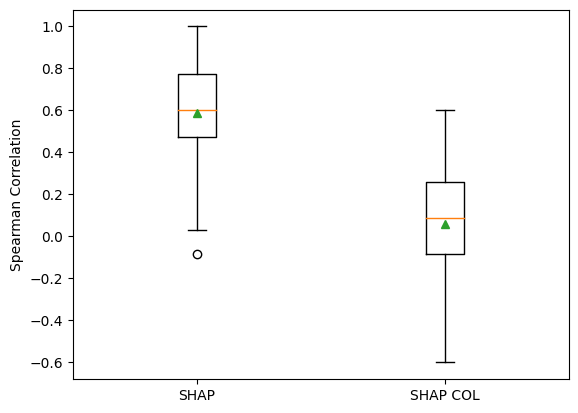
\includegraphics[width=.9\linewidth]{Figures/shap_colinearity.png}
%               \includegraphics[width=.9\linewidth]{Final_Figures/fig9b.png}%{Figures/shap_spearman_colinear.png}
%               \caption{}%Spearman rank correlations of signed feature importance magnitudes from LIME and SHAP against the true ranking from $\mathcal{G}$.}
%                \label{fig:shap_colinear}
%             \end{subfigure}
            
%             \caption{violin plots of 100 Spearman rank correlations of feature importance magnitudes given by LIME (left) and SHAP (right) data when explaining $\mathcal{G}_{\text{colinear}}$ and $\mathcal{G}^*$ directly. The 100 feature importance values are obtained by explaining the outcomes for 100 applicants in the test set.}
%             \label{fig:lime_shap_colinear}
%         \end{figure}

    
%     %We claim that this difficulty should be reduced as the data size increases. To test this, we simulate loan approval data sets of sizes $N=100,1000,10000,100000$, and train and explain models on each data set. We claim in particular that the roles of credit score and age in the explanations will become more accurate as $N$ increases. 



%     %Experiment setup for fenglu   
%     %Consider two correlated features A and B such that A has a larger impact on loan approval than B does. These features have a Pearson correlation of $r^2$ and VIF scores of $VIF$. We hypothesize that if we simulate loan approval data sets of sizes $N=100,1000,10000,100000$, then if we train and explain models on each data set, the roles of A and B in the explanations will become more accurate as $N$ increases. 
    
%     % do experiment with loan approval data with 2 correlated features and N small and N big to show the effects of the 2 correlated features can be disentangled for large enough N
    
%         %\textcolor{blue}{I'm not satisfied with the results of my experiments}
%         \paragraph{Non-confounding Redundant Features}
%         \label{sec:non_confounding_redundancy}
%          A redundant feature is also collinear; what distinguishes non-confounding redundancy from collinearity as in the previous section is that the redundant feature should receive 0 importance. 
%          To illustrate the problematic nature of nonconfounding redundant features, consider if in addition to the \emph{credit score} feature which uses a FICO scoring model, we had another credit score feature \emph{credit score 2} from another data analytics company which happened to report the FICO credit score plus a constant in order to flatter its users. Assuming that the second credit score is computed using the FICO credit score, the two features are correlated and \emph{credit score} is the causal ancestor of \emph{credit score 2}. In such a case, it is not clear that both should be given non-zero importance; the presence of the \emph{credit score 2} feature may dilute the degree to which a post hoc explainer suggests that \emph{credit score} has a causal effect on the loan approval probability. Moreover, \emph{credit score 2} is not a confounder because it is not a causal ancestor of another feature and does not causally affect loan approval. 
         
%          We test the influence of a redundant feature by setting $\mathcal{G}^*$ to be the same as the $\mathcal{G}^*$ from the previous experiment and setting $\mathcal{G}_{\text{redundancy}}^k$ to add to $\mathcal{G}^*$ a \emph{credit score 2} equal to credit score $+ k \epsilon$ where $k$ is varied from $.2$ to $1.0$ and $\epsilon \sim \mathcal{N}(0,20)$. Without \emph{credit score 2} present, the average and standard deviation of importance for \emph{credit score} for LIME are $.127\pm.007$ and for SHAP are $.102\pm .068$. After adding the redundant \emph{credit score 2} feature, the importance of \emph{credit score} is reduced for both LIME and SHAP and \emph{credit score 2} gets a positive importance of comparable size to that of \emph{credit score}. Furthermore, Figure \ref{fig:lime_shap_noise} shows that as the standard deviation of $\epsilon$ increases, the importance of \emph{credit score} goes down on average and the importance of \emph{credit score 2} increases on average. 

%          This experiment demonstrated that presence of a redundant feature can reduce the importance of its causal ancestor. This phenomenon is problematic, especially when the causal relationships underlying the data are not completely understood. Reduction of the importance of a feature by a feature it causes may cause the ranking of features obtained from an explainer to be incorrect.
         
%          %Without the redundant feature, LIME always perfectly ranks the features, whereas with a redundant feature LIME's mean Spearman Rank correlation against the true ranking is reduced to about .8 for all $k$. \textcolor{blue}{need to add figure for this}. LIME consistently allocates \emph{credit score 2} a non-zero importance value, while SHAP allocated \emph{credit score 2} no importance for all $k$. The variance of the noise present in the redundant feature evidently does not significantly affect explanation quality. 
        
%         \begin{figure}
%           \begin{subfigure}[t]{.4\textwidth}
%             \centering
%             \includegraphics[width=\linewidth]{Final_Figures/fig10a.png}%{Figures/lime_noise_1.png}
%             %\caption{LIME importance of credit score}
%           \end{subfigure}
%           \hfill
%           \begin{subfigure}[t]{.4\textwidth}
%             \centering
%             \includegraphics[width=\linewidth]{Final_Figures/fig10b.png}%{Figures/lime_noise_2.png}
%             %\caption{LIME importance of credit score 2}
%           \end{subfigure}
        
%           \medskip
        
%           \begin{subfigure}[t]{.4\textwidth}
%             \centering
%             \includegraphics[width=\linewidth]{Final_Figures/fig10c.png}%{Figures/shap_noise_1}
%             %\caption{SHAP importance of credit score}
%           \end{subfigure}
%           \hfill
%           \begin{subfigure}[t]{.4\textwidth}
%             \centering
%             \includegraphics[width=\linewidth]{Final_Figures/fig10d.png}%{Figures/shap_noise_2}
%             %\caption{SHAP importance of credit score 2}
%           \end{subfigure}
%         \caption{Violin plots of LIME/SHAP importances for credit score and credit score 2 by varying the standard deviation of the noise added to credit score 2.}
%         \label{fig:lime_shap_noise}
%         \end{figure}

        

    
%     \paragraph{Unobserved Confounding Features}
%         Complications also arise when unobserved confounding features are present. In our data, social support is an unobserved confounder of the cosigner feature. Increased social support increases the likelihood of having a cosigner, but there is no way to measure or observe social support in reality.  %The SHAP documentation \citep{dillon21becareful} shows that because an unobservable \emph{product need} confounds an observed feature \emph{bugs reported}, \emph{bugs reported} gets a positive SHAP. This would suggest making the software product more buggy would increase the likelihood of customers renewing their subscription to the service. Thus, failure to account for unobserved confounders may lead post hoc explainers to suggest the existence counter-intuitive or nonsensical phenomena. 
        
%         To illustrate the effects of unobserved confounders on explanation quality, we compare the ability of LIME and SHAP to recover the true rankings of features according to $\mathcal{G^*}$ where social support is not a factor at all and according to an MLP $\mathcal{M}$ trained on data produced by $\mathcal{G}_{\text{confounded}}$, which has social support that confounds the characteristics of the cosigner and credit score. The data generated by $\mathcal{G}^*$ only include age, sex, cosigner, credit utilization, credit inquiries, and credit score, and makes all features pairwise independent. Loan approval is determined using a linear combination of all the features. The data set generated by $\mathcal{G}_{\text{confounded}}$ includes the same features as the first, except that it adds social support as an unobserved confounder of the cosigner feature. Loan approval is then determined using a linear combination of age, sex, cosigner, credit utilization, credit inquiries, credit score, and social support. We assume that social support has 0 importance in both $\mathcal{G}^*$ and $\mathcal{M}$.%$ so that feature rankings are directly comparable between the two.

%         Having constructed $\mathcal{G}^*$ and $\mathcal{G}_{confounded}$ such that they differ only by the presence of a single unobserved confounder, we use violin plots to illustrate how the confounder affects explanations. In particular, we show the effect of the confounder on the feature importance of the cosigner feature. For both $\mathcal{G}^*$ and $\mathcal{G}_{\text{confounded}}$, \emph{ the cosigner} follows intuition by having a positive relationship with the likelihood of loan approval. When explaining 100 loan approvals/denials from $\mathcal{G}^*$ on the test set, both LIME and SHAP treat \emph{cosigner} such that, ignoring outliers, the importance distribution consists of only positive values. Figure \ref{fig:lime_shap_cosigner} shows, notably, that when \emph{cosigner} gets confounded by social support, SHAP begins to give it negative importance values. Without confounding and ignoring outliers, the Shapley values of \emph{cosigner} were between approximately.05 and.15. Once confounded, the range shifts to -.05 and .05.   %That is, we produce violin plots of Spearman Rank correlations of LIME and SHAP feature importance magnitude rankings against the true rankings from $\mathcal{G}^*$ and $\mathcal{G}_{confounded}$. Figure \ref{fig:lime_shap_confounder} shows that, for both LIME and SHAP, the distribution of Spearman rank correlations in the presence of the confounder is strictly lower than the distribution of Spearman rank correlations without confounders. 
        
        
        
%                 \begin{figure}[ht!]
%             \centering
%             \begin{subfigure}{.5\textwidth}
%               \centering
%               \captionsetup{justification=centering}
%               \includegraphics[width=.9\linewidth]{Final_Figures/fig11a.png}%{Figures/lime_cosigner.png}
%               %\caption{Spearman rank correlations of ranked feature importance magnitudes from LIME against the true ranked magnitudes from $\mathcal{G}$.}
%                \label{fig:lime_confounder}
%             \end{subfigure}%
%             \begin{subfigure}{.5\textwidth}
%               \centering
%                \captionsetup{justification=centering}
%               \includegraphics[width=.9\linewidth]{Final_Figures/fig11b.png}%{Figures/shap_cosigner.png}
%               %\caption{}
%                \label{fig:shap_cosigner}
%             \end{subfigure}
            
%             \caption{Violin plots of feature importance values for \emph{cosigner} from LIME and SHAP for cases when \emph{cosigner} is confounded and unconfounded.}
%            \label{fig:lime_shap_cosigner}
%         \end{figure}


    
       
% \subsubsection{Stage 2 Issues}
%     \label{sec:stage_2_issues}
% % \textcolor{red}{3\/13\/23 to show that stage 1 issues are not the only reason that cause the incorrectness, this section will also remove the controversial features , and make M = G (use LIME to explain G) and show that even if the bb model is perfect and the features are perfect, the explanations still have problems.}

%     %Discuss the problem with model-agnostic post hoc explainers in general
%     Having shown that the two most popular post hoc explainers can provide misleading explanations, we now investigate how the deficiencies of post hoc explainers could affect the business community in particular. We conclude that it is unrealistic to expect that model-agnostic post hoc explainers to provide explanations that do not substantially misrepresent the truth. As we will show in the next section, users can still be misled even in optimal conditions where causaul inference conditions are satisfied by the training data and $\mathcal{M}$ is highly accurate. This being the case, we explore opportunities for mitigation in Section \ref{sec:mitigation}.

% \subsubsection{Stage 2 Issues: Unreliable Explanations Even in Optimal Conditions}
%     \label{sec:optimal_conditions}
%     To facilitate fruitful usage of post hoc explainers so far, we presupposed that $\mathcal{M}$ is a "good" approximator of $\mathcal{G^*}$ trained on data from $\mathcal{G^*}$ that satisfies reasonable assumptions for causal inference. Namely, the lack of missing, collinear, or confounded features. In all experiments so far, and indeed in most reasonable scenarios in practice, the data has not satisfied causal inference conditions. Therefore, we now investigate whether the issues identified in the previous sections disappear when 1) $\mathcal{M}$ is highly accurate and 2) the data from $\mathcal{G}$ has no missing, collinear, or confounded features.

%     %['Age', 'Sex', 'Utilization', 'Inquiries', 'Credit Score']
%     To satisfy the two aforementioned conditions, we construct a simpler version of our data set by only include age, sex, credit utilization, credit inquiries, and credit score, and making credit score independent of the other features. In this data set, loan approval is now determined from these five observed, independent, features.  We train $\mathcal{M}$ as an MLP that attains 99\% test set accuracy and an AUC of .98 and re-do our previous experiments testing the abilities of LIME and SHAP to correctly rank features by their importance.
    
%     Following our previous experiment, we first task LIME and SHAP with recovering the true ranking of feature importance magnitudes from $\mathcal{M}$ and $\mathcal{G}^*$ for 100 applicants. Figure \ref{fig:lime_shap_spearman_m_g} shows that, when explaining $\mathcal{M}$, LIME is never able to extract the true feature ranking but does get close with high consistency. SHAP also cannot recover the true feature importance rankings and additionally has more variance in the ranking distribution. When explaining $\mathcal{G^*}$ itself, LIME seems to be able to perfectly recover the true ranking order almost always. When explaining $\mathcal{G}^*$, SHAP can actually recover the true feature importance ranking, but with less consistency than LIME does. 

%     Our results considering signed importance values instead of magnitudes appear in \ref{fig:lime_shap_spearman_m_g_signed}. We see from Figure \ref{fig:lime_shap_spearman_m_g_signed} that the Spearman rank correlations of the ranks of the signed feature importance values given by LIME and SHAP when explaining $\mathcal{M}$ drop significantly compared to those obtained using feature importance magnitudes.  The lower tails of the ranking distributions also extend into the negative range, indicating that LIME and SHAP can supply rankings that correlate negatively with the true ranking. However, LIME is always able to produce the exact rankings when explaining $\mathcal{G}^*$. In contrast, the rankings of signed Shapley values from SHAP seem to be less accurate in general and more often than the rankings of Shapley value magnitudes.

%     %Figures \ref{fig:lime_shap_spearman_m_g} and \ref{fig:lime_shap_spearman_m_g_signed} suggest that if one just wants to know the relative importance of features to a classifier \emph{and} the data the classifier was trained on satisfies conditions for causal inference, LIME and SHAP can be useful tools and will provide accurate feature rankings with high consistency. However, if one additionally wants to know how each feature affects the outcome variable, LIME and SHAP may not be useful unless you have access to the ground truth data generation model $\mathcal{G}^*$.

%            \begin{figure}[ht!]
%             \centering
%             \begin{subfigure}{.5\textwidth}
%               \centering
%               \includegraphics[width=.9\linewidth]{Final_Figures/fig12a.png}%{Figures/lime_spearman_mg_perfect.png}
%               %\caption{A subfigure}
%               \label{fig:lime_m_g}
%             \end{subfigure}%
%             \begin{subfigure}{.5\textwidth}
%               \centering
%               \includegraphics[width=.9\linewidth]{Final_Figures/fig12b.png}%{Figures/shap_spearman_mg_perfect.png}
%               %\caption{A subfigure}
%               \label{fig:shap_m_g}
%             \end{subfigure}
%             \caption{Violin plots of 100 feature importance values given by LIME (left) and SHAP (right) data when explaining an MLP $\mathcal{M}$ and when explaining $\mathcal{G}$ directly. The 100 feature importance values are obtained by explaining the outcomes for 100 applicants in the test set.}
%             \label{fig:lime_shap_spearman_m_g}
%         \end{figure}


%         \begin{figure}[ht!]
%             \centering
%             \begin{subfigure}{.5\textwidth}
%               \centering
%               \includegraphics[width=.9\linewidth]{Final_Figures/fig13a.png}%{Figures/lime_spearman_mg_perfect_signed.png}
%               %\caption{A subfigure}
%               \label{fig:lime_m_g_signed}
%             \end{subfigure}%
%             \begin{subfigure}{.5\textwidth}
%               \centering
%               \includegraphics[width=.9\linewidth]{Final_Figures/fig13b.png}%{Figures/shap_spearman_mg_perfect_signed.png}
%               %\caption{A subfigure}
%               \label{fig:lime_shap_g_perfect}
%             \end{subfigure}
%             \caption{Violin plots of 100 Spearman rank correlations of signed feature importance values given by LIME (left) and SHAP (right) data when explaining an MLP $\mathcal{M}$ and when explaining $\mathcal{G}$ directly. The 100 feature importance values are obtained by explaining the outcomes for 100 applicants in the test set.}
%             \label{fig:lime_shap_spearman_m_g_signed}
%         \end{figure}

% % REMOVED FOR CIST
% % \subsection{Attempted ``Mitigation'' Strategies for Incorrectness}
% % \label{sec:mitigation} %\textcolor{red}{move this to the end of section 4. this is the mitigation strategy for incorrectness}
% %     We propose several mitigation strategies. We show the relationship between the accuracy of $\mathcal{M}$ and the accuracy of LIME and SHAP's feature importance rankings to isolate the effects of $\mathcal{M}$ on LIME and SHAP. We used the local fidelity of LIME's linear surrogate models similarly to investigate its trade-off with stability. Finally, we check whether different averaging strategies might reduce the severity with which LIME and SHAP's feature importance rankings differ from those of $\mathcal{G^*}$. 


% % \subsubsection{Does High-Accuracy of $\mathcal{M}$ Imply High-Quality Explanations?}
% % \label{sec:m_fidelity}
% %     To answer this question, we used two strategies to control the accuracy of the model. One strategy is to assume that there is enough training data and control the accuracy of the model by varying its parameters. The other strategy is to change the accuracy of the model by varying the size of the training data set with the same model parameters. In our experience, differences in model accuracy due to both of these scenarios are common in the real world. \par
% %     Figures 15 to 17 show the performance of the metrics in Sections 4.1.1 to 4.1.3 under the two strategies, respectively. From Figure 15, we can find that the correlation of importance magnitude ranking increases accordingly as the accuracy of the model increases, regardless of the strategy adopted. And the effect of the first strategy is significantly better than that of the second strategy. However, unfortunately, realistically researchers may not have enough training data. Therefore, even though our experimental results show that the post hoc explainer can give a very good explanation in terms of importance magnitude ranking when a very good model is trained with enough data, this is almost non-existent in real life. From Figure 16 we see that no matter what strategy is adopted to improve the accuracy of the model, there is no large improvement in the signed ranking relevance as the accuracy of the model improves. In terms of recall, it can be seen from Figure 17 that although LIME and SHAP's recall improves with accuracy under both strategies, the improvement is very limited, with the improvement in recall averaging no more than 20\% when the accuracy is improved from about 55\% to 95\%.\par
% %     In summary, although the descriptive insights of post hoc explainers improve somewhat with model accuracy, and even in some extreme cases (sufficient data, good models, appropriate metrics) they can give very good descriptive insights, these improvements are more limited or difficult to generalize in the real world.\par
% %     Similarly, we considered the effect of model accuracy on prescriptive insights. We used the metrics in Section 4.2.2 to portray the effect of Dice on prescriptive insights. As can be seen in Figure 18, when the model accuracy improves from 55\% to 95\%, the success rate of counterfactual generation improves from 25\% to 50\%. Despite the degree of improvement in success rate, even the better models do not end up with very good prescriptive insights.

% %     \begin{figure}[ht!]
% %     \centering
% %         \begin{subfigure}{.48\textwidth}
% %               \centering
% %               \includegraphics[width=\linewidth]{Final_Figures/fig14a.png}%{Figures/feng_fig/acc_increase_iter_1.png}
% %               %\caption{A subfigure}
% %               \label{fig:acc_increase_metric1_strategy1}
% %         \end{subfigure}%
% %         \hfill
% %         \begin{subfigure}{.48\textwidth}
% %               \centering
% %               \includegraphics[width=\linewidth]{Final_Figures/fig14b.png}%{Figures/feng_fig/acc_increase_size_1.png}
% %               %\caption{A subfigure}
% %               \label{fig:acc_increase_metric1_strategy2}
% %         \end{subfigure}
% %         \hfill
% %     \caption{Line plots of 100 Spearman rank correlations of feature importance magnitude ranking given by LIME and SHAP when increasing $\mathcal{M}'s$ accuracy by changing model parameter strategy (left) and changing training size(right) strategy.}
% %     \label{fig:acc_increase_metric1}
% %     \end{figure}

% %         \begin{figure}[ht!]
% %         \centering
% %             \begin{subfigure}{.48\textwidth}
% %               \centering
% %               \includegraphics[width=\linewidth]{Final_Figures/fig15a.png}%{Figures/feng_fig/acc_increase_iter_2.png}
% %               %\caption{A subfigure}
% %               \label{fig:acc_increase_metric2_strategy1}
% %             \end{subfigure}%
% %             \hfill
% %             \begin{subfigure}{.48\textwidth}
% %               \centering
% %               \includegraphics[width=\linewidth]{Final_Figures/fig15b.png}%{Figures/feng_fig/acc_increase_size_2.png}
% %               %\caption{A subfigure}
% %               \label{fig:acc_increase_metric2_strategy2}
% %             \end{subfigure}
% %         \caption{Line plots of 100 Spearman rank correlations of signed feature importance magnitude given by LIME and SHAP when increasing $\mathcal{M}'s$ accuracy by changing model parameter strategy (left) and changing training size (right) strategy.}
% %         \label{fig:acc_increase_metric2}
% %         \end{figure}

% %         \begin{figure}[ht!]
% %         \centering
% %             \begin{subfigure}[h]{.48\textwidth}
% %                   \centering
% %                   \includegraphics[width=\linewidth]{Final_Figures/fig16a.png}%{Figures/feng_fig/acc_increase_iter_3_1.png}
% %                   %\caption{A subfigure}
% %                   \label{fig:acc_increase_metric3_strategy1_lime}
% %             \end{subfigure}%
% %             \hfill
% %             \begin{subfigure}[h]{.48\textwidth}
% %                   \centering
% %                   \includegraphics[width=\linewidth]{Final_Figures/fig16b.png}%{Figures/feng_fig/acc_increase_iter_3_2.png}
% %                   %\caption{A subfigure}
% %                   \label{fig:acc_increase_metric3_strategy1_shap}
% %             \end{subfigure}%
% %             \hfill
% %             \begin{subfigure}[h]{.48\textwidth}
% %                   \centering
% %                   \includegraphics[width=\linewidth]{Final_Figures/fig15c.png}%{Figures/feng_fig/acc_increase_size_3_1.png}
% %                   %\caption{A subfigure}
% %                   \label{fig:acc_increase_metric3_strategy2_lime}
% %             \end{subfigure}%
% %             \hfill
% %             \begin{subfigure}[h]{.48\textwidth}
% %                   \centering
% %                   \includegraphics[width=\linewidth]{Final_Figures/fig15d.png}%{Figures/feng_fig/acc_increase_size_3_2.png}
% %                   %\caption{A subfigure}
% %                   \label{fig:acc_increase_metric3_strategy2_shap}
% %             \end{subfigure}%
% %             \hfill
% %         \caption{Average recall of LIME(left) and SHAP(right) when increasing $\mathcal{M}'s$ accuracy by Changing model parameter strategy (top) and changing training size(botton) strategy.}
% %         \label{fig:acc_increase_metric3}
% %         \end{figure}


% % \begin{figure}[ht!]
% %     \centering
% %     \includegraphics[width=0.8\textwidth]{Final_Figures/fig17.png}%{Figures/feng_fig/acc_dice.png}
% %     \caption{Percentages of times DiCE was able to produce true counterfactuals for rejected applicants for Models with different accuracy.}
% %     \label{fig:dice_acc}
% % \end{figure}

% % \subsubsection{Does High-Fidelity of $\mathcal{E}$ Imply High-Quality Explanations?} 
% % \label{sec:e_fidelity}
% %     Post hoc explainers like LIME only approximate, but are not the decision-making processes themselves. Thus, when LIME trains a linear model to reproduce a local prediction, it is possible that the predicted value from LIME does not equal to the original model output. The mismatch between the black-box to be explained and the post hoc explainer is called the ``fidelity'' of an explainer \cite{laugel18defining}. Thus, it is natural to wonder whether increasing the overall fidelity of the model could improve the correctness of the explanations. That is, if an explainer can reproduce the predictions of a black-box model with 100\% accuracy, does that mean the explanation is correct and faithful?

% %             To answer this question, we first use an experiment to empirically investigate the relationship between the fidelity of LIME and the quality of its explanations of the ground truth data generator and of an MLP trained on the data. To do this, we vary LIME's kernel width parameter 50 times and for each kernel width, we construct LIME explanations of 1000 training data points from the simulated ad-clicking data set. For each kernel width, we associate a measure of fidelity equal to the proportion of the 1000 training points that the local LIME explainers classified the same as the model being explained when using a threshold of 0. We compute the fidelity for each kernel width as the proportion of the 1000 points that LIME's surrogate model classifies correctly. We also associate each kernel width with the average Spearman Rank Correlations with the explained model's ranking, taken over the LIME 1000 explanations. Plotting the fidelity measurements versus the average Spearman Rank Correlations reveals that there is no statistically significant relationship between LIME's fidelity and the correctness of its explanation. This is true for the case when LIME is explaining the ground truth data generation model and when LIME is explaining an MLP trained on the data. 


            
% \section{Rashomon Effect of Post Hoc Explanations}
%         A Rashomon effect of post hoc explainers refers to the phenomenon in which post hoc explainers provide a set of explanations that is inconsistent in the sense that one explainer contradicts itself, two explainers contradict each other, or both. Both attributive and counterfactual explainers may provide differing explanations of the same input. This may or may not be a problem depending on the use-case. For example, one may want to choose from among a set of explanations based on which explanations most align with domain knowledge. Indeed, the ability to produce diverse counterfactuals for the same input is one of the main features of DiCE. However, we are concerned with cases when the multiplicity of explanations is problematic. Examples of such cases could be when one does not have domain knowledge and does not know what explanation to pick, and/or when there are explanations that contradict each other. In any case, picking a single explanation may be difficult because there is no way to know what explanation is the best. 
        
%         Due to the Rashomon effect, researchers cannot just choose one explainer or one explanation. \cite{han22which} introduces a no-free-lunch theorem for post hoc explainers, stating that no one explainer can always provide the best explanation. This is because for every explainer, there must exist a neighborhood around a data point to be explained such that \emph{another} explainer is a better approximator of the ground truth in that neighborhood. \cite{kommiya21towards} also showed that different explainers are either (implicitly) solving entirely different optimization problems or solving the same (or a similar one) differently. They defined two objectives $\alpha$ and $\beta$ for which different post hoc explainers choose to optimize and do so differently. $\alpha$ captures the ability for an explainer to utilize features that are \emph{necessary} for the outcome being explained. $\beta$ captures the ability for an explainer to utilize features that are \emph{sufficient} to cause the outcome being explained. \cite{kommiya21towards} shows that LIME and SHAP take different approaches for optimizing $\beta$, while counterfactual methods optimize for $\alpha$. Thus, theory suggests that we should not expect LIME, SHAP, or DiCE to be consistent with each other. There will always be a Rashomon effect when using post hoc explainers.

% \subsection{Cause of Rashomon Effect} 
%         \subsubsection{Stage 2 Issues: Inconsistencies Between Explainers}
%         \label{sec:conflict_between}
%             %To motivate the use of multiple post hoc explainers, we show that they may explain the same outcome in different ways with differing degrees of accuracy. 
%             Conflicting explanations between explainers can lead to a conundrum for researchers. On one hand, users may have to choose from among conflicting explanations and suffer the consequences if they pick a bad explanation. On the other, because each explanation has some modicum of truth, managerial insights drawn from a single explainer may be incomplete or incorrect. Notably, this is increasingly likely as the data dimension increases \citep{kommiya21towards}. To justify these claims, we demonstrate the inconsistency of LIME and SHAP on the simulated loan data set.%, then show how the inconsistency grows when larger and larger feature subsets are used on the Iranian Housing data set. 
    
%             Given a trained MLP $\mathcal{M}$ on the loan data, we would like to investigate how different LIME and SHAP explanations of the same points are. To this end, we sample 100 test data points and obtain feature rankings according to the importance allocated to them by both LIME and SHAP. Figure \ref{fig:lime_shap_spearman_together} shows that, on average, LIME and SHAP most often have rankings are nearly uncorrelated. The first quartile of Spearman rank correlations between LIME and SHAP rankings is about -.3, meaning that LIME and SHAP had negatively correlated rankings about a quarter of the time. 

%             % REWORK NEXT TO PARAGRAPHS
%             These results suggest once more that post hoc explainers should be used with caution. In particular, more than one explainer should be used because different explainers may provide conflicting explanations. It is up to the user to attempt to either somehow leverage multiple explanations or identify which is the most sensible using their domain knowledge (and taking care to avoid the biases outlined in Section \ref{sec:human_explainer_interaction}. 

%             Being that it is impossible in practice to know what explainer is the most correct, this experiment illustrates the importance of leveraging multiple explainers to maximize the likelihood that correct insights are drawn. Although \citep{kommiya21towards} recommended this, to the best of our knowledge, exactly how to leverage multiple explainers is an open problem. We treat this problem in Section \ref{sec:mitigation}.
            

%             \begin{figure}[ht!]
%                 \centering
%                 \includegraphics[width=.5\textwidth]{Figures/lime_shap_spearman_together.png}
%                 \caption{Violin plot of Spearman Rank Correlations between LIME and SHAP explanations of 100 points}
%                 \label{fig:lime_shap_spearman_together}
%             \end{figure}



%     \subsubsection{Stage 2 Issues: Inconsistency from the Same Explainer}
%             \label{sec:conflict_within}
%              Both LIME and SHAP are designed such that there may be variability in explanations of the same individual between runs. However, because we noticed that SHAP is fairly robust, this section focuses on LIME. 
%              Hyperparameters and sampling are causes of inconsistency between multiple runs of LIME. LIME depends on a random seed, the number of samples to generate around the point to explain, the kernel function (default Gaussian), the kernel width defining the size of the neighborhood around the point to explain, and the hyperparameters of the surrogate model (e.g. LASSO vs RIDGE). 
             
%              LIME explains a black box's output at a point by solving an artificial regression problem inside a neighborhood of that point. Changing the design matrix of a regression problem changes the resulting estimator. LIME's hyperparameters change the design matrix, so we should not expect its explanations to be consistent across runs. \cite{rahnama19shift} formalizes this claim by studying the data and labels shift present in the artificial data created by LIME and showing that even for small sample sizes, LIME causes significant data/label shift.           \cite{visani21stability} studied the role of LIME's kernel width and ridge penalty on the consistency of explanations on models trained on credit risk data. They confirm that low ridge penalties and large kernel widths lead to inconsistent explanations for the same individual. Inconsistency was quantified using two metrics that they developed, called the Variability Stability Index (VSI) and the Coefficients Stability Index (CSI). Note that \citep{visani21stability} uses the term instability to refer to inconsistent explanations for the same individual with the same hyperparameters whereas we use the definition of instability from \citep{molnar2019}.
             
             
%              %Moreover, the quality with which SHAP approximates Shapley values is determined by the $nsamples$ hyperparameter, which represents the number of training data samples used to evaluate the black box model when explaining a prediction.



%             To get an idea of how LIME and SHAP explanations are affected by hyperparameters in a business context, we examine the importance of an applicant's credit score given by different combinations of models and explainers. We evaluate consistency by checking 1) if LIME and SHAP can at least give credit score feature importance values with consistent signs and 2) if those values stay relatively consistent regardless of random seeds or hyperparameters. Simultaneously, we investigate how the accuracy of $\mathcal{M}$ affects explanations. %Section \ref{sec:rashomon_overfitting} will give an overview of how instability affects LIME and SHAP.%and results in inconsistent explanations. 

%             We found that feature importance signs were relatively consistent when explaining only one individual. In particular, if we reuse the same experimental setup as in Section \ref{sec:pipeline_demo} and construct importance value histograms by using LIME and SHAP to explain the predictions of the same applicant 100 times by different models $\mathcal{M}$ and different instantiations of LIME and SHAP with different hyperparameter settings and record the importance of the applicant's credit score (the data set's known most important feature), credit score almost always gets a consistently signed feature importance value by both explainers.  Figure \ref{fig:lime_imp_rejected} shows that for each model, regardless of accuracy, LIME almost always gives credit score a negative feature importance sign. But it also admits the possibility of giving credit score a small positive feature importance sign even for more accurate models. Figure \ref{fig:shap_imp_rejected} shows that SHAP is robust to its random seed being changed, but gives credit score larger Shapley values as the accuracy of $\mathcal{M}$ increases.




% \begin{figure}[ht!]
% \centering
%     \begin{subfigure}{.48\textwidth}
%           \centering
%           \includegraphics[width=\linewidth]{Final_Figures/fig19a.png}%{Figures/lime_imp_rejected.png}
%           \caption{Violin plots of credit score importance from different combinations of $\mathcal{M}$ and LIME}
%           \label{fig:lime_imp_rejected}
%     \end{subfigure}%
%     \hfill
%     \begin{subfigure}{.48\textwidth}
%           \centering
%           \includegraphics[width=\linewidth]{Final_Figures/fig19b.png}%{Figures/shap_imp_rejected.png}
%           \caption{Violin plots of credit score importance from different combinations of $\mathcal{M}$ and SHAP}
%           \label{fig:shap_imp_rejected}
%     \end{subfigure}
% \caption{Illustration of how the importance of credit score changes as the accuracy of $\mathcal{M}$ changes and how the hyperparameters of the explainers explaining $\mathcal{M}$ change. We vary the kernel width and random seed of LIME. We only vary the random seed of SHAP. To produce the models $\mathcal{M}$, we initialize an MLP with a consistent random state (if this is not done, the results are quite erratic; the clear downward trend of the violin plots does not appear.) and train for $1,2,3...$ up to $15$ iterations}.
% \label{fig:lime_shap_imp_rejected}
% \end{figure}



%         Having demonstrated that the same applicant can indeed get different explanations from LIME depending on LIME's parameters, we now discuss what those explanations actually look like. We discuss how explanations change by keeping LIME's random seed constant but varying the kernel width from $.05\sqrt{\#Features}$ to $\sqrt{\#Features}$ with a step size of $.05\sqrt{\#Features}$. When the kernel width is larger than $.15\sqrt{\#Features}$, the feature ranking from LIME is constant (and incorrect), stating that credit inquiries, number of months since last delinquent payment, and credit utilization are the top three most important features. For smaller kernel widths, the three most important features are some permutation of credit inquiries, number of months since the last delinquent payment, and credit utilization. The remaining features are also shuffled. LIME's explanations are both incorrect and inconsistent.

%     \subsubsection{Stage 2 Issues: Inconsistencies leading to conflicting insights}
%         \label{sec:conflicting_insights}
%         In this subsection, we make concrete the claims of the previous two subsections on the inconsistency of explainers. First, we show that LIME and SHAP do not present a consistent narrative for why applicants are rejected. Then, we exhibit a multitude of explanations for why our trained MLP predicts that an applicant in the simulated loan data set is predicted to be rejected.  We adopt the same experimental setup as in Section \ref{sec:pipeline_demo} and provide different explanations of the same rejected individual. %Importantly, we noticed that not using standardized data worsens the inconsistency of LIME. 

%     This section explores the consequences of using post hoc explainers when standard assumptions for causal inference are not satisfied.  Standard assumptions on data include 1) that all relevant features are included in the data, that all features in the data set must be 2) pairwise-independent of each other 3) independent of any unobserved confounding features, and 4) the treatment of interest temporally precedes the outcome. This section has two main conclusions. First, depending on the explainer used and its settings, actionable recourse using counterfactuals may be ineffective. Second, if conditions 1-4 are violated, feature importance from post hoc explainers cannot be trusted. 

%     We illustrate our conclusions using hypothetical scenarios based on loan approval data and loan approval data. The first scenario we consider is that of when someone would like direction on how to change their risk assessment from high to low by making minimal changes to their lifestyle. Intuitively, one would assume that perturbation of the most important features LIME and SHAP identify could help them become low risk and receive a line of credit, but unfortunately we do not find this to be the case.

%     Our experiments with the loan approval data indicate that 1) managers are unlikely to be able to ascertain the true relative importance of features from post hoc explainers and 2) if their data does not satisfy the conditions for causal inference, as it likely wouldn't for any realistic business data, post hoc explainers should not be used. 


% % REMOVED FOR CIST???
% \subsection{Attempted ``Mitigation'' Strategy for Rashomon Effect} 
% \label{sec:mitigation}


% \subsubsection{Averaging Explanations of One Explainer}
%     Section \ref{sec:conflict_within} demonstrated the multiplicity of explanations due to random seeds and hyperparameters, so it is natural to wonder if multiple explanations can be aggregated to provide an explanation that tends to be the most accurate. To this end, we check if taking king the mean and median of feature importance values from LIME and SHAP taken over combinations of random seeds and hyperparameters reveals a useful aggregation strategy. \par
%     We compare the ability of LIME and SHAP in many places in the previous sections. Both have unreliable explanations. A natural thought is whether averaging their explanations would make the final explanation more reliable. To test this hypothesis, we averaged the explanations with LIME and SHAP for the same batch of instances.\par
% Figure 22 and Figure 23 show the differences between LIME, SHAP, and their averaged explanation for the metrics in Sections 4.1.1 and 4.1.3, respectively (we cannot use the metrics in Section 4.1.2 because LIME and SHAP do not have the same meaning for the metric and cannot be averaged for them).\par
% As we can see in Figures 22 and 23, the performance of the average explanation falls in between the explanations of LIME and SHAP. This suggests that if we really cannot tell exactly which explainer works better, then averaging their results is a safer way, but in the end the results will not be better. In short, averaging the results of different explainers does not make the final result better, it only makes it not the worst.

% \begin{figure}[ht!]
%     \centering
%     \includegraphics[width=.5\textwidth]{Final_Figures/fig20.png}%{Figures/feng_fig/average_lime_shap_1_v1.png}
%     \caption{Violin plot of Spearman Rank Correlations of feature importance magnitude ranking by LIME, SHAP and LIME+SHAP}
%     \label{fig:lime_shap_Spearman_together}
% \end{figure}

% \begin{figure}[ht!]
%     \centering
%     \includegraphics[width=.5\textwidth]{Final_Figures/fig21.png}%{Figures/feng_fig/average_lime_shap_3_v1.png}
%     \caption{Average recall of LIME, SHAP and LIME+SHAP}
%     \label{fig:lime_shap_Spearman_together}
% \end{figure}


% \begin{figure}[ht!]
% \centering
%     \begin{subfigure}{.48\textwidth}
%           \centering
%           \includegraphics[width=\linewidth]{Final_Figures/fig22a.png}%{Figures/feng_fig/lime_0_v1.png}
%           %\caption{A subfigure}
%           \label{fig:avering_within_lime_metric1}
%     \end{subfigure}%
%     \hfill
%     \begin{subfigure}{.48\textwidth}
%           \centering
%           \includegraphics[width=\linewidth]{Final_Figures/fig22b.png}%{Figures/feng_fig/shap_0_v1.png}
%           %\caption{A subfigure}
%           \label{fig:avering_within_shap_metric1}
%     \end{subfigure}
% \caption{Violin plots of 100 Spearman rank correlations of feature importance magnitude ranking given by LIME(left) and SHAP(right) when averaging different numbers of model results}
% \label{fig:avering_within_experlainers_metric1}
% \end{figure}


% \begin{figure}[ht!]
% \centering
%     \begin{subfigure}{.48\textwidth}
%           \centering
%           \includegraphics[width=\linewidth]{Final_Figures/fig23a.png}%{Figures/feng_fig/lime_1_v1.png}
%           %\caption{A subfigure}
%           \label{fig:avering_within_lime_metric2}
%     \end{subfigure}%
%     \hfill
%     \begin{subfigure}{.48\textwidth}
%           \centering
%           \includegraphics[width=\linewidth]{Final_Figures/fig23b.png}%{Figures/feng_fig/shap_1_v1.png}
%           %\caption{A subfigure}
%           \label{fig:avering_within_shap_metric2}
%     \end{subfigure}
% \caption{violin plots of 100 Spearman rank correlations of signed feature importance rankings given by LIME(left) and SHAP(right) when averaging different numbers of model results}
% \label{fig:avering_within_experlainers_metric2}
% \end{figure}

% \begin{figure}[ht!]
% \centering
%     \begin{subfigure}{.48\textwidth}
%           \centering
%           \includegraphics[width=\linewidth]{Figures/feng_fig/lime_2_v1.png}
%           %\caption{A subfigure}
%           \label{fig:avering_within_lime_metric3}
%     \end{subfigure}%
%     \hfill
%     \begin{subfigure}{.48\textwidth}
%           \centering
%           \includegraphics[width=\linewidth]{Figures/feng_fig/shap_2_v1.png}
%           %\caption{A subfigure}
%           \label{fig:avering_within_shap_metric3}
%     \end{subfigure}
% \caption{Average recall given by LIME(left) and SHAP(right) when averaging different numbers of model results}
% \label{fig:avering_within_experlainers_metric3}
% \end{figure}

% \subsubsection{Averaging Explanations across Explainers}
%     Since \citep{kommiya21towards} demonstrated that feature importance rankings differed significantly across different explainers, we also seek a useful aggregation strategy for explanations from LIME, SHAP, and DiCE. We attempt to find such a strategy by averaging feature importance rankings from LIME, SHAP, and DiCE by averaging explanations from each of these over their hyperparameters and random seeds. Specifically, we sample 100 applicants from the data, produce a set of LIME explanations of these applicants by varying the random seed, and produce another set by varying the kernel width. Likewise, for each applicant, we produce sets of SHAP explanations created by varying SHAP's random seed and $nsamples$ parameter.


% \paragraph{Discussion} 
% In addition to demonstrating that post hoc explanations from LIME can be incorrect, inconsistent, and misleading to business researchers in Sections 4 and 5, we proposed and tested some intuitive mitigation strategies that leverage multiple explainers in an effort to combat the Rashomon effect in Section \ref{sec:mitigation}. To the best of the authors' knowledge, the first call for such mitigation strategies appeared \citep{kommiya21towards}. Our mitigation strategies suggested that averaging the results of an ensemble of explanations does not give significantly better explanation on average than individuals in the ensemble. However, \textcolor{red}{we also suggest more research to be done on this topic. Perhaps a bagging method exists that would be successful}. In any case, we emphasize that outside of employing causal inference methods, the best solution for business researchers is to use inherently interpretable models instead of blax violines~\citep{rudin18stop}. We owe the caveat in the previous sentence to the fact that inherently interpretable models, like black boxes, do not necessarily learn the causal mechanisms that exist in their training data. Therefore, when it is sufficient to understand the relationships learned by a machine learning model (and not the relationships in data), we recommend to use an inherently interpretable machine learning model. When causal relationships underlying a data set need to be identified, causal inference methodology should be employed. post hoc explainers are not a suitable option in either scenario. 


% REMOVED FOR CIST
% \section{Discussion and Conclusion}
%     \label{sec:discussion}

%     \subsection{Summary of Findings}
%         Using simulated loan application data sets, we produced ground truth application approval mechanisms $\mathcal{G}$ along with MLP approximators $\mathcal{M}$ trained on $\mathcal{G}$ and investigated how well popular post hoc explainers can produce correct descriptive and prescriptive insights into $\mathcal{G}$. This investigation was motivated by the need to assess the utility of post hoc explainers to business researchers and managers. 

%         We claim that for the sake of finding correct descriptive business insights about an ML model using post hoc explainers, the following issues are cause for caution. First, the two most popular post hoc explainers, LIME and SHAP, cannot reliably rank features in order of their ground truth importance and how they affect the target variable. Second, users face a Rashomon effect for explanations because not only do LIME, SHAP, and DiCE each produce different explanations for the same outcome, but LIME may produce self-contradictory explanations of the same outcome. It is up to the user to decide what explanation to choose, based on their own domain knowledge.

%         Our main finding regarding prescriptive insights is that LIME, SHAP, and DiCE seem to only be of use for actionable recourse a minority of the time. When tasked with generating new application profiles for denied loan applicants, those new application profiles would be approved by $\mathcal{G}$ less than 50\% of the time. %\textcolor{blue}{May need to be removed!! We showed that... DiCE, a counterfactual explainer (as opposed to an attributive one like LIME and SHAP) was always able to produce new application profiles for rejected loan applicants that would lead to approval in our experiments (for a sufficiently small sparsity parameter). }For DiCE, if we restrict the range of feature variations (within one standard deviation) and the number of features allowed to vary, it can only provide prescriptive insights to a small number of denied applicants.
        
%     \subsection{On Mitigation Strategies}
%         We proposed some intuitive mitigation strategies consisting of techniques to construct aggregate explanations that are better on average than individual explanations. These strategies include averaging the results across interpreters (Section 5.2.1) and averaging the results under different hyperparameters of the same interpreter (Section 5.2.2).\par
% Our results show that the first strategy does not make the averaged results better, but at most makes the final results not the worst. The second strategy, on the other hand, only makes the explanations more stable, but does not improve them.\par

%     \subsection{General Recommendations}
%         Although post hoc explainers have some intrinsic issues that affect their reliability, users can still influence the quality of explanations. We outline recommendations for each step in the use of post hoc explainers.
        
%         First, users should keep in mind the studies claiming that data scientists may misuse a post hoc explanation due to a fundamental misunderstanding of the explainer (by, e.g., having an incorrect understanding of what a Shapley value is) and/or inflicting their biases onto the explanation. Users should ensure that they have a complete understanding of how explainers they intend to use work and how their biases may affect their understanding of the explanation. Ideally, XAI researchers would also develop explainers that are not so prone to user error. 
        
%         Second, before even beginning model development, users should attempt to understand the causal graph associated with their problems and employ statistical tests of unconfoundedness assumptions. With this knowledge, users need to decide whether it is worthwhile to use post hoc explainers instead of randomized experiments. If so, the data should be preprocessed to remove redundant features. If applicable, the causal descendant of a collinear pair of causally linked features should be removed. Confounders should be controlled for if possible. 

%         Third, because we found that the accuracy/AUC of $\mathcal{M}$ was related to explanation quality, variability, and the ability to construct true counterfactuals, we propose that extra effort in making highly accurate models that generalize well is important. Overfitting is especially detrimental because the complexity of the decision boundary of $\mathcal{M}$ contributes to the instability of the explainer. After all, even a perfect explainer for a model which is highly locally nonlinear must be unstable. Thus, needless complexity in a decision boundary due to overfitting could cause an explainer of the decision function to be unstable when it should not be.  

%         Finally, when constructing explanations of a model, averaging the results of different explainers may be a good choice because our experiments suggest that average explanations are not strictly worse than their component explanations. Moreover, constructing an average explanation over a set of explainer hyperparameters improves stability but does not result in a strictly better explanation than the component explanations.     
% write about trying mitigations but note that they aren't super useful
% take out stuff about randomized experiments
% no ADVOCATING
\section{Conclusion}
Throughout this paper we have identified various consequences of the use of model agnostic post hoc explainers that could lead to incorrect business and managerial insights. We classify the issues into two categories, incorrectness and multiplicity.  On the surface, model-agnostic post hoc explainers are attractive because they are easy to use and applicable to any model with any data set. But evidence from the machine learning community and this paper both suggest that post hoc explanations, although valuable, are not a panacea for extracting business insights from black-box models. Because they not only have intrinsic issues which can make them unreliable, but also may be interpreted by humans, they are not always trustworthy.  

Our results suggest, e.g., that it is possible that businesses or customers trying to improve upon some outcome could waste time and resources adjusting for an irrelevant feature that LIME or SHAP implied were important. In addition, simple mitigation strategies are not effective and do not guarantee reliable outcomes. Thus, due to the stakes involved with understanding business problems, we urge the business community to use post hoc explainers with great caution. When using them, business researchers should keep in mind the problems related to incorrectness and inconsistency laid out in this paper. %Post hoc explanations should not be assumed to be correct, but rather taken as evidence that the proposed explanation may be true.

        


% References here (outcomment the appropriate case)

% CASE 1: BiBTeX used to constantly update the references
%   (while the paper is being written).
%\bibliographystyle{informs2014} % outcomment this and next line in Case 1
%\bibliography{<your bib file(s)>} % if more than one, comma separated

% CASE 2: BiBTeX used to generate mypaper.bbl (to be further fine tuned)
%\input{mypaper.bbl} % outcomment this line in Case 2

%If you don't use BiBTex, you can manually itemize references as shown below.

\clearpage

\bibliographystyle{informs2014}
\bibliography{refs}

\clearpage

% dimensions finds only 206 but indexes preprints
% scopus finds over 400 but doesn't index preprints
%% preprint not necessary
% need to ensure that the papers are actually explaining a black box
% e.g. add

\section{Appendix}

    \begin{figure}[ht!]
        \centering
        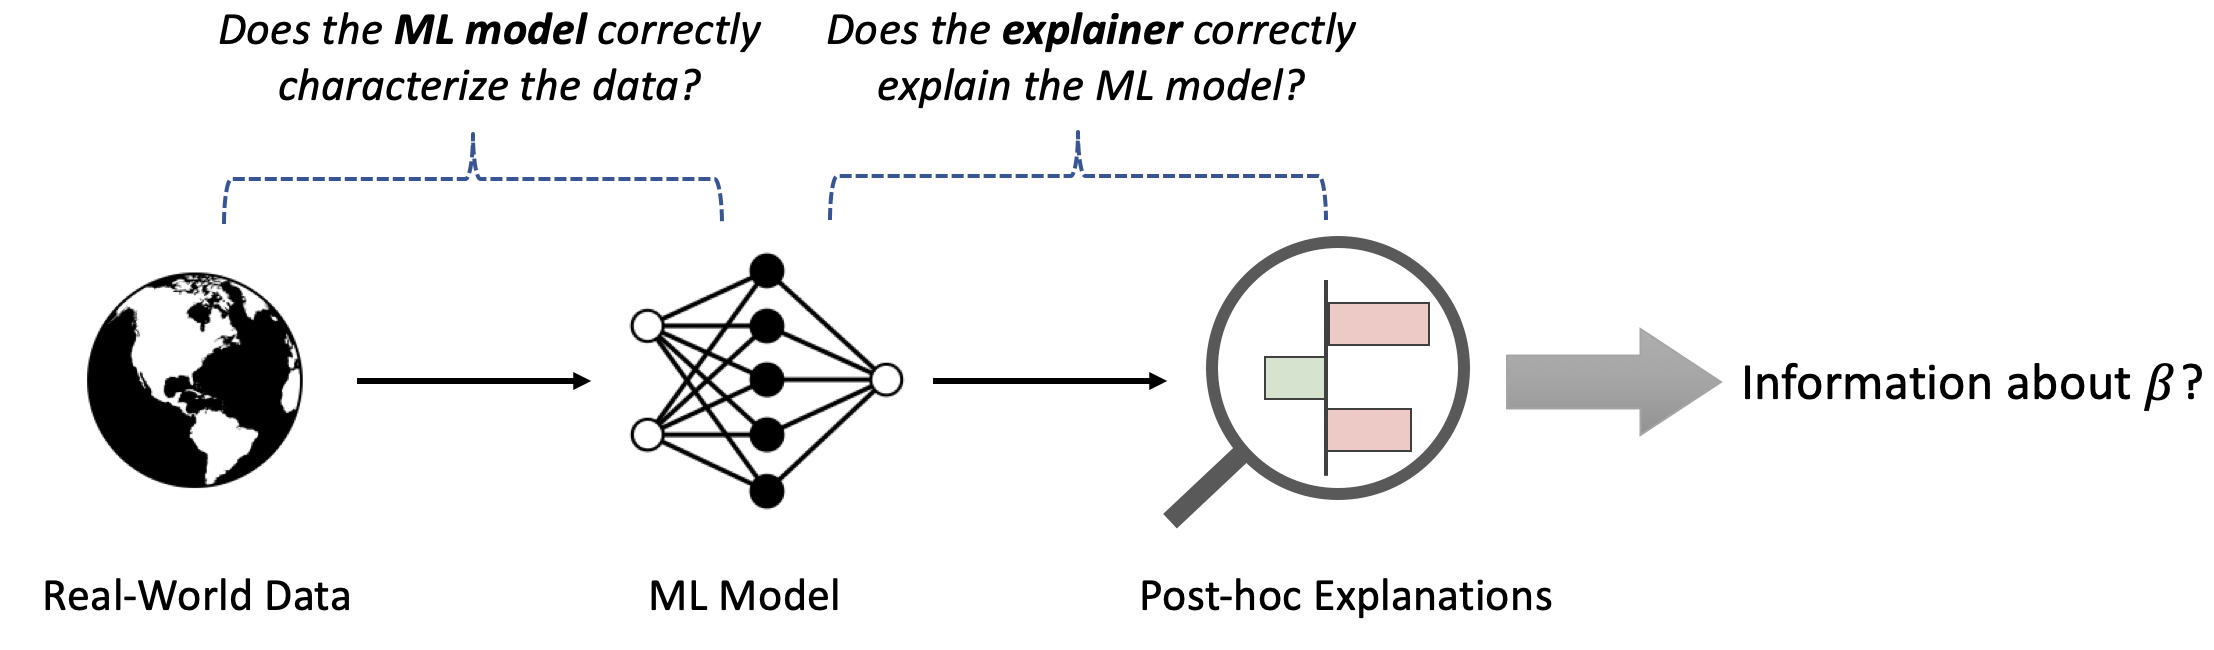
\includegraphics[width = \textwidth]{Figures/pipeline.png}
        \caption{Prediction Insight Pipeline: the pipeline of using post hoc explainers to obtain managerial insights in business research.}
        \label{fig:pipeline}
    \end{figure}

 \begin{table}[h]
 \small
\centering
\caption{Description of features for simulated loan data.   }
\resizebox{\textwidth}{!}{%
\begin{tabular}{|l|l|l|l|}
\hline
\textbf{Feature} & \textbf{Explanation}                           & \textbf{Formula}       & \textbf{Comment}                             \\ \hline
%\rowcolor[gray]{.9}
Age              & Applicant Age                                   & Uniform(18,100)        &                                              \\ \hline
%\rowcolor[gray]{.9}
Sex              & Applicant Sex                                   & Bernoulli(.5)          &                                              \\ \hline
Married          & Applicant Marital Status                        & Bernoulli(.5)          &                                              \\ \hline
Social Support   & 0 = no support, 1 = perfectly supported        & Uniform(0,1)           & Not observable                               \\ \hline
Cosigner         & Indicator of presence of loan cosigner         & Bernoulli(.5)          & Depends on social support and marital status \\ \hline
%Economy          & Health of the economy in the customer's region & Uniform(0,1)           &                                %              \\ \hline
Income           & Applicant Income                                & Normal(40,000, 30,000) & %Colinear with Economy 
\\ \hline
%\rowcolor[gray]{.9}
Utilization      & Proportion of total credit utilized            & Uniform(0,1)           & %Colinear with Economy 
\\ \hline
Delinquencies    & Number months since of last deliquent payment                   & Uniform(0,25)          &                                              \\ \hline
%\rowcolor[gray]{.9}
Inquiries         & Number of credit inquiries                     & Uniform(0,6)           &                                              \\ \hline
%\rowcolor[gray]{.9}
Credit Score\footnote{Credit scores based on a partial FICO credit scoring model \citep{ligons_fico} are calculated as follows: $\text{credit score} = 650 + (10 + 2.5\cdot \text{credit history}) + (70 - 15 \cdot \text{Inquiries}) + (35 - 4 \cdot \text{delinquencies}) + (105 - 100 \cdot \text{Utilization})$}     & Credit score based on FICO scoring             & Given below            & Depends on inquiries, delinquencies, and utilization.                                             \\ \hline
\end{tabular}%
}
%Note that for demonstration purposes, Section \ref{sec:pipeline_demo} experiments use all features but the unobserved social support variable.}
\label{tab:simulated}
\end{table}

                % \begin{figure}[ht!]
                % \centering
                %     \begin{subfigure}[t]{.48\textwidth}
                %           \centering
                %           \includegraphics[width=\linewidth]{Figures/lime_shap_spearman_magnitude.png}%{Figures/feng_fig/acc_increase_iter_1.png}
                %           \caption{Spearman rank correlations of ranked feature importance magnitudes from LIME and SHAP against the true ranked magnitudes from $\mathcal{G}$.}
                %           \label{fig:lime_shap_Spearman_magnitude}
                %     \end{subfigure}%
                %     \hfill
                %     \begin{subfigure}[t]{.48\textwidth}
                %           \centering
                %           \includegraphics[width=\linewidth]{Figures/lime_shap_topk.png}%{Figures/feng_fig/acc_increase_size_1.png}
                %           \caption{Average recall of LIME and SHAP for top K most important features to $\mathcal{G}$ when explaining $\mathcal{M}$. Vertical lines indicate the 95\% confidence interval.}
                %           \label{fig:avg_recall}
                %     \end{subfigure}
                %     \hfill
                % \caption{Results of experiments evaluating how well LIME and SHAP can provide descriptive insights. We measure how well their feature rankings align with the true global importance from $\mathcal{G}$ and how often they can identify the top $K$ features.}
                % \label{fig:sec4figs}
                % \end{figure}


\begin{figure*}[!h]
\centering
    \begin{subfigure}[t]{0.3\textwidth}
    \centering
    \includegraphics[width=\linewidth]{Figures/lime_shap_spearman_signed.png}%{Figures/feng_fig/acc_increase_iter_1.png}
                          \caption{Spearman rank correlations of ranked feature importance values from LIME and SHAP against the true ranking from $\mathcal{G}$.}
                          \label{fig:lime_shap_Spearman_signed}
\end{subfigure}\hfill
\begin{subfigure}[t]{0.3\textwidth}
    \centering
    \includegraphics[width=\linewidth]{Figures/lime_shap_topk.png}%{Figures/feng_fig/acc_increase_size_1.png}
                          \caption{Average recall of LIME and SHAP for top K most important features to $\mathcal{G}$ when explaining $\mathcal{M}$. Vertical lines indicate the 95\% confidence interval.}
                          \label{fig:avg_recall}
\end{subfigure}\hfill


\caption{Results of experiments evaluating how well LIME and SHAP can provide descriptive insights. We measure how well their feature rankings align with the true global importance from $\mathcal{G}$ and how often they can identify the top $K$ features.}
\label{fig:sec4figs}
\end{figure*}



                

\begin{figure*}[!h]
\centering
    \begin{subfigure}[t]{0.3\textwidth}
    \centering
    \includegraphics[width=\textwidth]{Figures/lime_recourse_k.png}
    \caption{Success rate of actionable recourse performed by perturbing up to 4 of the most important features identified by LIME.} \label{fig:lime_recourse_k}
\end{subfigure}\hfill
\begin{subfigure}[t]{0.3\textwidth}
    \centering
    \includegraphics[width=\textwidth]{Figures/shap_recourse_k.png}
    \caption{Success rate of actionable recourse performed by perturbing up to 4 of the most important features identified by SHAP.} \label{fig:shap_recourse_k}
\end{subfigure}\hfill
 \begin{subfigure}[t]{0.3\textwidth}
    \centering
    \includegraphics[width=\textwidth]{Final_Figures/fig8a.png}
    \caption{Success rate of actionable recourse performed by allowing DiCE to perturb up to 4 mutable features.} \label{fig:dice_recourse_k}
\end{subfigure}

\caption{Success rates of actionable recourse attempted for 100 rejected applicants using LIME, SHAP, and DiCE.}
\label{fig:recourse_figs}
\end{figure*}


            % \begin{figure}[ht!]
            %     \centering
            %     \includegraphics[width=.5\textwidth]{Figures/lime_shap_spearman_together.png}
            %     \caption{Spearman Rank Correlations between LIME and SHAP explanations of 100 points}
            %     \label{fig:lime_shap_spearman_together}
            % \end{figure}

            %     \begin{figure}
            %               \centering
            %               \includegraphics[width=.5\textwidth]{Final_Figures/fig14a.png}%{Figures/feng_fig/acc_increase_iter_1.png}
            %               \caption{Line plot of 100 Spearman rank correlations of feature importance magnitude ranking given by LIME and SHAP when increasing $\mathcal{M}'s$ accuracy. Vertical lines indicate the 95\% confidence interval of the Spearman correlation for given accuracies.}
            %               \label{fig:acc_increase_metric1_strategy1}
            %     \end{figure}

\begin{figure}
    \centering
    \begin{minipage}[t]{0.3\textwidth}\centering%
        \includegraphics[width=\textwidth]{Figures/lime_shap_spearman_together.png}
                \caption{Spearman Rank Correlations between LIME and SHAP explanations of 100 points.}
                \label{fig:lime_shap_spearman_together}
    \end{minipage}\hfill
    \begin{minipage}[t]{0.3\textwidth}\centering%
        \includegraphics[width=\textwidth]{Final_Figures/fig14b.png}
                          \caption{Line plot of 100 Spearman rank correlations of feature importance value rankings given by LIME and SHAP when increasing $\mathcal{M}'s$ accuracy.}%Vertical lines indicate the 95\% confidence interval of the Spearman correlation for given accuracies.}
                          \label{fig:acc_increase_metric1_strategy1}
    \end{minipage}\hfill
    \begin{minipage}[t]{0.3\textwidth}\centering%
        \includegraphics[width=\textwidth]{Figures/lime_ranking_dist.png}
  \caption{Violin plots of feature rankings from LIME computed over 10,000 combinations of kernel widths and random seeds.}
  \label{fig:lime_rankings}
    \end{minipage}
\end{figure}

                

\begin{figure*}[!h]
\centering
    \begin{subfigure}[t]{0.3\textwidth}
    \centering
    \includegraphics[width=\textwidth]{Final_Figures/fig23a.png}
  \caption{Violin plots of 100 Spearman rank correlations of LIME feature importance  rankings when averaging different numbers of model results.}\label{fig:avering_within_lime_metric1}
\end{subfigure}\hfill
\begin{subfigure}[t]{0.3\textwidth}
    \centering
    \includegraphics[width=\textwidth]{Final_Figures/fig23b.png}
  \caption{Violin plots of 100 Spearman rank correlations of SHAP feature importance rankings when averaging different numbers of model results.}
  \label{fig:avering_within_shap_metric1}
\end{subfigure}\hfill
 \begin{subfigure}[t]{0.3\textwidth}
    \centering
    \includegraphics[width=\textwidth]{Final_Figures/fig20.png}
  \caption{Violin plots of Spearman rank correlations of feature importance rankings by LIME, SHAP and LIME+SHAP.}
  \label{fig:averaging_lime_shap}
\end{subfigure}

\caption{Results of mitigation strategies involving averaging the results of one explainer and averaging the results of two explainers together.}
\label{fig:mylabel}
\end{figure*}
%%%%%%%%%%%%%%%%%
\end{document}
%%%%%%%%%%%%%%%%%

